\documentclass[12pt]{article}


\usepackage{graphicx}
\graphicspath{{origin graphs/}}
\usepackage{hyperref}
\hypersetup{colorlinks=true, citecolor=blue, linkcolor=blue, urlcolor=blue}
%\usepackage[duipsnames]{xcolor}
\usepackage{caption}
%\usepackage{subcaption}
\usepackage{apacite}
                                                 
\usepackage{pdfpages}



\begin{document}

\includepdf[pages=1]{Front_page}
%\maketitle
%\clearpage
\tableofcontents
\clearpage
%\listoffigures
%\clearpage

\begin{abstract}
In this paper we have have tried to study the production and spectroscopic investigation of Mercury and Radon isotopes using complete fusion reactions neutron evaporation residues and multi-nucleon transfer reaction at the mass-separator MASHA installed on the beam line of Cyclotron U-400M at Flerov Laboratory of Nuclear Reactions (FLNR) in Joint Institute for Nuclear Research (JINR), Dubna, Russia. The isotopes produced in complete fusion reactions\\
 $^{148}Sm(^{40}Ar,xn)^{188-x}Hg$, $^{166}Er(^{40}Ar,xn)^{206-x}Rn$ and multi-nucleon transfer reaction $^{48}Ca$ + $^{242}Pu$ were passed through the magneto-optical system of MASHA setup with charge state Q=+1 and were separated on the basis of their mass to charge ratio. For the detection of these isotopes, a position sensitive Si detector is used. Further, the experimental data obtained were analysed and spectroscopic investigations were carried out.
\end{abstract}

\section{INTRODUCTION}
The MASHA (Mass Analyzer of Super Heavy Atoms) setup has been designed as a mass-separator with the resolving power of about 1700, which allows mass identification of superheavy nuclides. The setup uses the solid ISOL (Isotope Separation On-Line) method. The work on the project means the analysis of real data collected from the experiments of complete fusion reactions neutron evaporation residues $^{40}Ar$ + $^{148}Sm$ $\rightarrow$ $^{188-x}Hg$ + $xn$,\\ $^{40}Ar$ + $^{166}Er$ $\rightarrow$ $^{206-x}Rn$ + $xn$  and multi-nucleon transfer reaction\\ $^{48}Ca$ + $^{242}Pu$ using the $\alpha$-decay chains from the position sensitive Si detector.\\
\\
Here, we have analyzed the experimental data from the above stated reactions to calculate the masses of identified isotopes(which are results of the above nuclear reactions), their half life, Alpha Branching Ratio (ABR), energy of $\alpha$-decay $(E_a)$ and their probability to decay with a specific amount of energy. Using these experimental data we have plotted one dimensional $\alpha$-decay energy spectrum and its peak analysis was performed. We have also tried to obtain a fit for all the isotopes (Parent Nuclei) and their $\alpha$-decay products (called Daughter Nuclei) using Gaussian fitting function. Further, using the 1D histograms ($\alpha$-decay energy spectrum) we have obtained a heatmap (two dimensional energy-position graph) for the isotopes.
\clearpage

\section{LAYOUT OF MASHA SETUP AND ITS MAIN PARTS}
The MASHA setup is shown in fig \ref{Scheme of the MASHA setup: D1, D2, D3a, D3b – dipole magnets, Q1, Q2, Q3 – quadrupole lenses, S1, S2 – sextupole lenses.}. It consists of a Target Box with a Hot Catcher, an ECR Ion Source, Magneto-Optical System (or mass to charge ratio analyzer), and a Position Sensitive based Si Detector (Detection and Control System). It also consists of an intermediate plane (F1) and for detailed monitoring of isotopes, an additional strip detector has been installed at this middle plane. Each part of the MASHA facility is explained in detail below. For in-depth knowledge on MASHA setup, one can refer this paper \cite{vedeneev2017current}.

\begin{figure}[h]
\centering
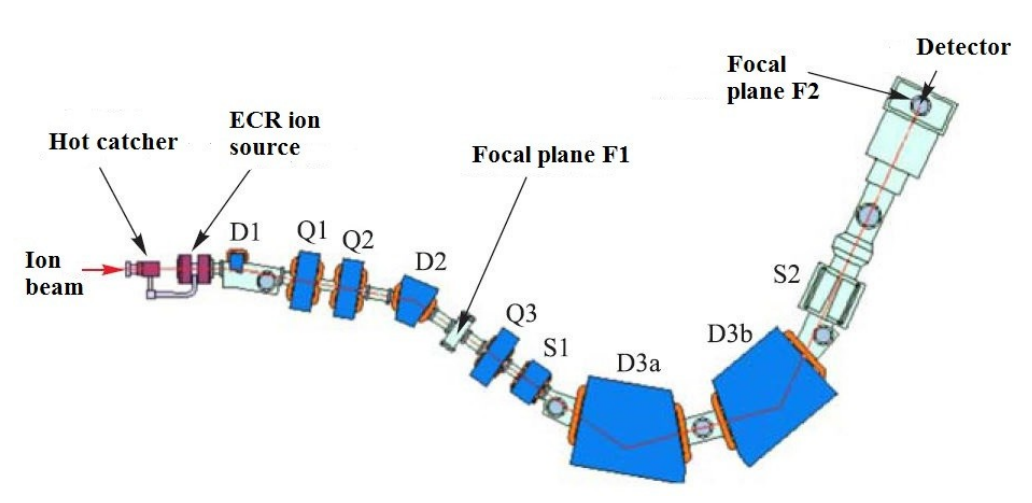
\includegraphics[scale=0.6]{MASHA.png}
\caption{\textbf{Scheme of the MASHA setup: D1, D2, D3a, D3b – dipole magnets, Q1, Q2, Q3 – quadrupole lenses, S1, S2 – sextupole lenses.}}
\label{Scheme of the MASHA setup: D1, D2, D3a, D3b – dipole magnets, Q1, Q2, Q3 – quadrupole lenses, S1, S2 – sextupole lenses.}
\end{figure}

\subsection{TARGET BOX}
The target box consists of a rotating disc divided into 6 sectors, which are sputtered with target material (or materials) as shown in fig \ref{Rotating target disc present in target box.}. The disc rotates with a frequency of 25Hz\cite{georgiadis2020production}. The high energetic projectile particle ejected from U-400M cyclotron collides with the target material to induce some kind of nuclear reaction. The products of the nuclear reaction are stopped by the hot catcher.
\begin{figure}[h]
\centering
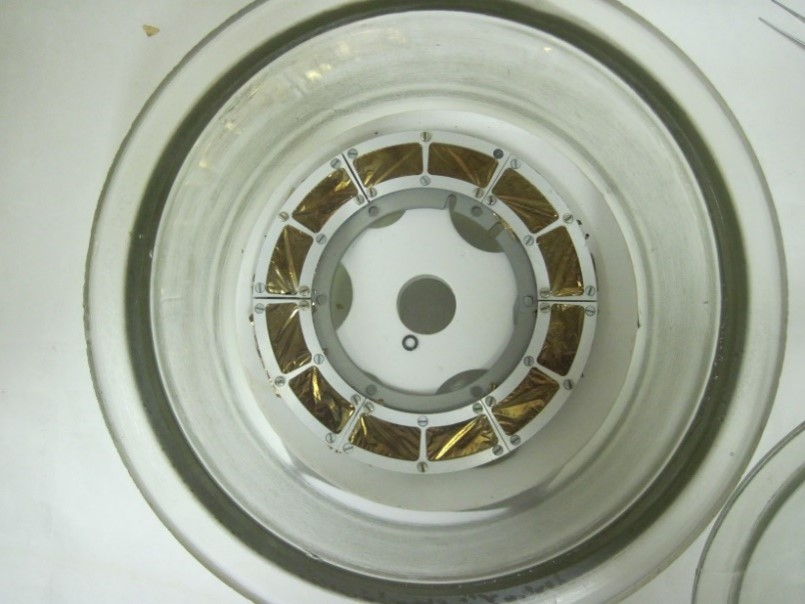
\includegraphics[scale=0.8]{Rotating Target.jpg}
\caption{\textbf{Rotating target disc present in target box.}}
\label{Rotating target disc present in target box.}
\end{figure}

\subsection{HOT CATCHER}
The diagram of hot catcher is shown in fig \ref{Hot Catcher consists of two components-poly-graphene heater & absorber material.}. It consists of mainly two components, one is poly-graphene heater and the other one is absorber material. The latter is usually made up of thin film of graphite or carbon nanotubes heated by the former upto a temperature of $1800-2000^oC$. As depicted in figure the absorber is installed in front of the heater at a distance of 2 mm along the beam axis of MASHA\cite{mamatova2019study}. 
\begin{figure}[h]
\centering
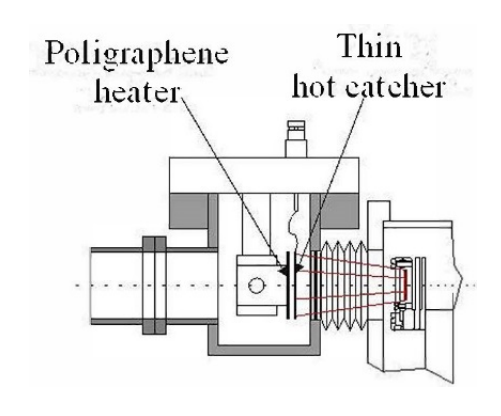
\includegraphics[scale=0.5]{HC.png}
\caption{\textbf{Hot Catcher consists of two components - poly-graphene heater \& absorber material.}}
\label{Hot Catcher consists of two components-poly-graphene heater & absorber material.}
\end{figure}
The products of the nuclear reaction is stopped by the absorber material, vaporized to gaseous form and are passed to the ECR ion source. Fig \ref{Complete schematic of target box with hot catcher.} shows the complete schematic of target box with hot catcher.

\begin{figure}[h]
\centering
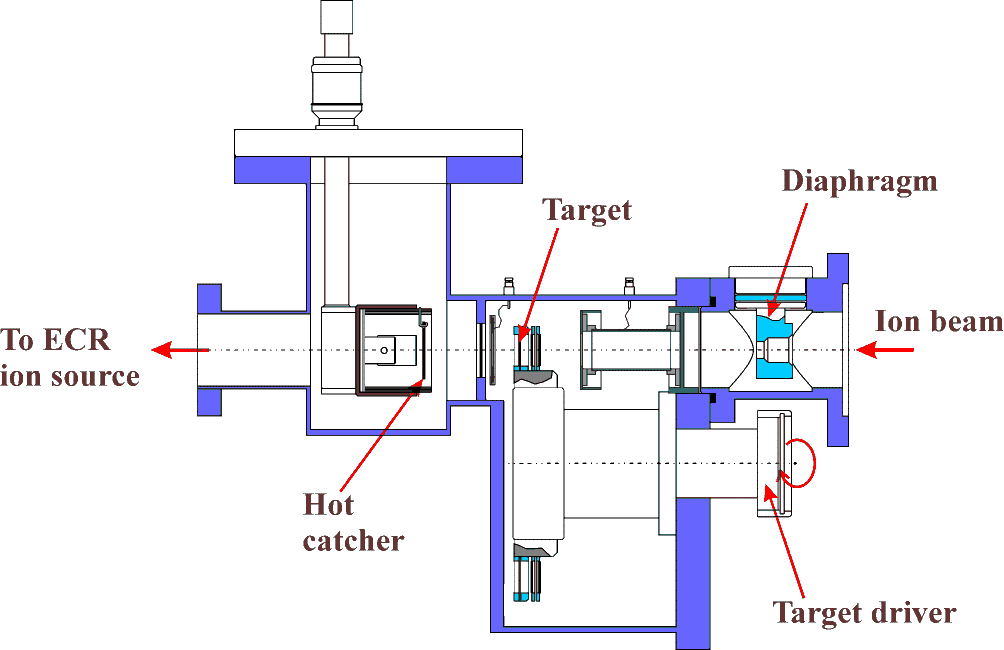
\includegraphics[scale=0.95]{TBHC.png}
\caption{\textbf{Complete schematic of target box with hot catcher.}}
\label{Complete schematic of target box with hot catcher.}
\end{figure}

\subsection{ECR ION SOURCE}
The ECR (Electron Cyclotron Resonance) ion source with a microwave oscillation frequency of 2.45 GHz\cite{rodin2014separation}, acts as an ionization chamber of MASHA spectrometer. It ionizes the atoms of gaseous isotopic products of nuclear reaction to a charge state Q=+1, and accelerates them to an energy of 48 KeV using three electrode system. The ionized atoms gets converted to beam and are then separated by magneto-optical system of the MASHA spectrometer.

\subsection{MAGNETO-OPTICAL SYSTEM}
The magneto-optical system separates the beam of ions on the basis of their mass to charge ratio. The magnetic separation of heavy nuclei is performed using four dipole magnets(D1, D2, D3a, D3b), three quadrupole lenses (Q1, Q2, Q3) and two sextupole lenses (S1, S2) as shown in fig \ref{Scheme of the MASHA setup: D1, D2, D3a, D3b – dipole magnets, Q1, Q2, Q3 – quadrupole lenses, S1, S2 – sextupole lenses.} Once, the heavy nuclei gets separated they are then detected at different strips of position sensitive Si detector.

\subsection{POSITION SENSITIVE Si DETECTOR}
The position sensitive Si detector is a multiple detector system used to detect the separated heavy nuclei. It is installed at the focal plane (F2) of the MASHA setup. A clear view of the position sensitive Si detector is shown in fig \ref{Position sensitive Si detector. 1-front detector, 2-upper detector, 3-lower detector, 4-lateral detector.}. The front detector has an area of 240x35 $mm^2$ and it consists of 192 strips. The upper and lower detector consists of 64 strips while the left and right lateral detector consists of 16 strips. Each strip has a width of 1.25 mm and each detector has a thickness of 0.3 mm\cite{rodin2014masha}.

\begin{figure}[h]
\centering
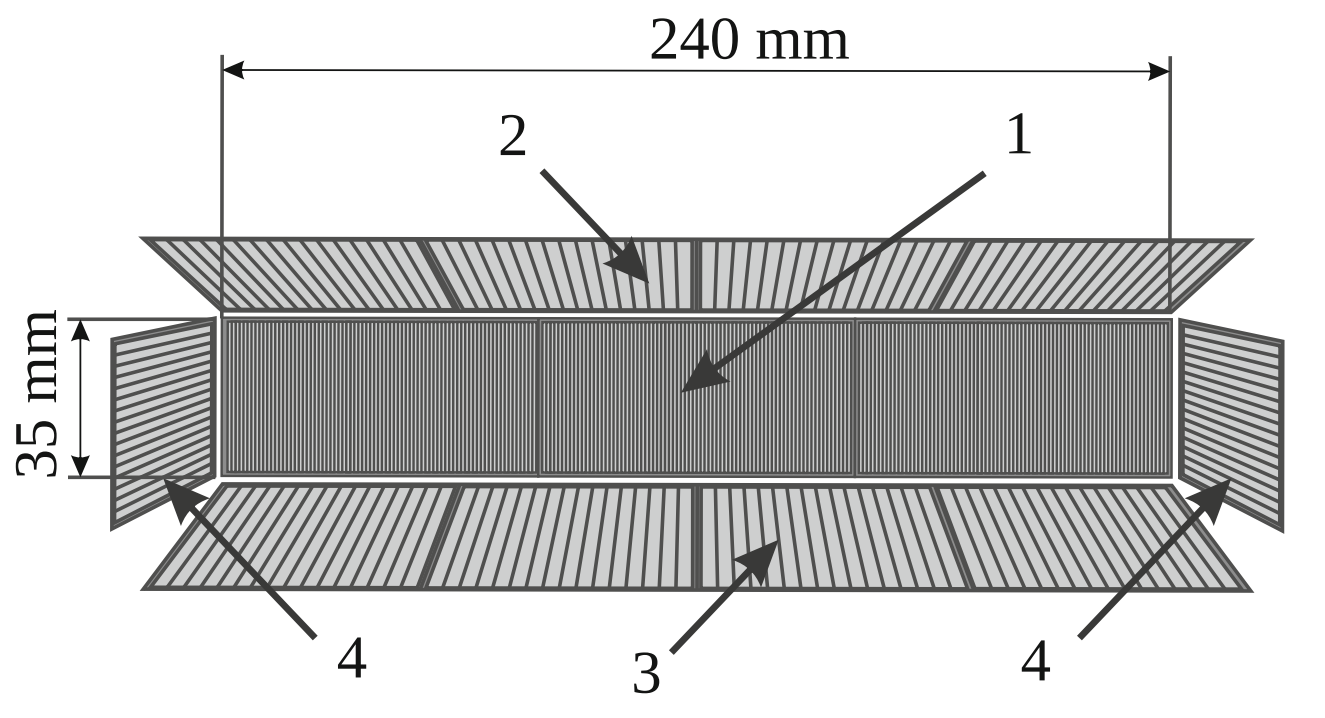
\includegraphics[scale=.4]{Detector.png}
\caption{\textbf{Position sensitive Si detector. 1-front detector, 2-upper detector, 3-lower detector, 4-lateral detector.}}
\label{Position sensitive Si detector. 1-front detector, 2-upper detector, 3-lower detector, 4-lateral detector.}
\end{figure}

\section{SCIENCE BEHIND THE EXPERIMENT}
The test experiments carried out at FLNR are:
\begin{enumerate}
\item $^{40}Ar$ + $^{148}Sm$ $\rightarrow$ $^{188-x}Hg$ + $xn$
\item $^{40}Ar$ + $^{166}Er$ $\rightarrow$ $^{206-x}Rn$ + $xn$
\item $^{48}Ca$ + $^{242}Pu$ $\rightarrow$ (Any element whose Z varies from 20-114)
\end{enumerate}
The first and second nuclear reactions are complete fusion reactions neutron evaporation residues. In such types of reactions the product nucleus formed has no. of protons exactly equal to no. of protons of projectile particle + no. of protons of target nucleus. Here, all the nucleons participate in the reaction. While the third one is a Multi-Nucleon Transfer Reaction (MNTR). In such nuclear reactions different nuclides can be formed whose atomic no. ranges from atomic no. of projectile particle to sum of atomic nos. of projectile particle + target nucleus. This means not all nucleons participate in this reaction and can lead to formation of any possible product. The N/Z ratio of product nucleus can be higher or lesser than than the optimal ratio required for its stability (i.e. It can be proton rich or neutron rich).\\
\\
The U-400M cyclotron installed at FLNR, JINR is used to accelerate projectile particle ($^{40}Ar$ \& $^{48}Ca$) to a very high velocity, with an energy \~ 240 MeV (for $^{40}Ar$ + $^{148}Sm$) and with energy \~ 198 MeV ($^{40}Ar$ + $^{166}Er$). The high energetic projectile particle enters into the MASHA setup and induce a nuclear reaction by colliding with target material sputtered in rotating disc present in target box of MASHA facility. The products of nuclear reaction are isotopes of Hg (for $^{40}Ar$ + $^{148}Sm$)  and Rn (for $^{40}Ar$ + $^{166}Er$ and $^{48}Ca$ + $^{242}Pu$) which are stopped by the absorber material of hot catcher.\\
\\
The absorber material is generally made up of thin film of graphite or carbon nanotubes which is heated to around $1800-2000^oC$ by means of IR radiations coming out from poly-graphene heater as well as by a direct current passing through the absorber. This absorber stops the isotopic products of nuclear reaction, vaporizes them and their respective atoms diffuses through this absorber material into the vacuum volume of the hot catcher. Moving along the vacuum pipe, they reach the ECR ion source.
This ECR ion source acts as an ionization chamber of MASHA setup where the atoms of gaseous isotopic products gets ionized to charge state Q=+1 and further they are accelerated with the help of three electrode system. (The three electrode system consists of one positive electrode, one negative electrode and one more negative electrode. Hence, an electric field is established from positive electrode to negative electrode. So, when a charged particle (here, ion) moves in the direction of electric field, it gets accelerated.\\
\\
The product isotopes are then separated by their M/Q ratio in the magneto-optical system of MASHA setup and at last they reach to the focal plane (F2) of the position sensitive Si detector and are detected at different strip numbers. (i.e. different isotopes are detected at different strip numbers).\\
\\
Now, the science is that the separated heavy nuclei undergoes
$\alpha$-decay to produce daughter nuclei and it's exactly the alpha particles (with different energies) given out by both parent nucleus and its daughter nuclei which are detected at unique strip nos. of position sensitive Si detector. The detector used is a hybrid pixel detector of the TIMEPIX type, with high resolution and sensitivity which can detect even a single $\alpha$ or $\beta$ particle. So, from the experimental data, we plot $\alpha$-decay energy spectrum for those strips where an isotope was detected. From this spectrum ($\alpha$-decay energy Vs. No. of counts) we analyze the prominent peaks and calculate their $\alpha$-decay energy ($E_a$) values. The base peak with maximum no. of $\alpha$ particles (with common energy) is our point of interest as it could be any one of the separated nuclei. Now, using the table of nuclides, we find which isotope (of product of nuclear reaction) undergoes $\alpha$-decay with energy very close to it. That particular isotope will be the one detected at a unique strip no. Ones, the isotope gets detected, its mass, alpha branching ratio, daughter nuclei can easily be investigated using the table of nuclides. In the same way we detect all the isotopes of an element which is the product of a nuclear reaction.\\
\\
In this work, we have also analyzed a two dimensional energy-position graph (called heatmap) for all three test experiments. It gives a clear understanding that which isotope is detected at which strip no. and corresponding to that particular isotope, how many alpha particles (counts) are detected with a common energy. This common energy is the energy of $\alpha$-decay of that isotope.

\section{SPECTROSCOPIC INVESTIGATION OF\\ MERCURY ISOTOPES USING FULL-FUSION REACTION $^{148}Sm(^{40}Ar,xn)^{188-x}Hg$}
The complete fusion reaction of $^{148}Sm(^{40}Ar,xn)^{188-x}Hg$ was carried out at MASHA setup. The target material sputtered in rotating disc was $^{148}Sm$ and the products of the nuclear reaction were isotopes of Hg. However, only long-lived isotopes of Hg were detected whose half-life was greater than average separation time (1.8±0.3 s) used by ISOL method for this reaction.


\clearpage

\subsubsection{PRODUCTION OF $^{180}Hg$}
\begin{figure}[h]
\centering
 \begin{subfigure}
\centering
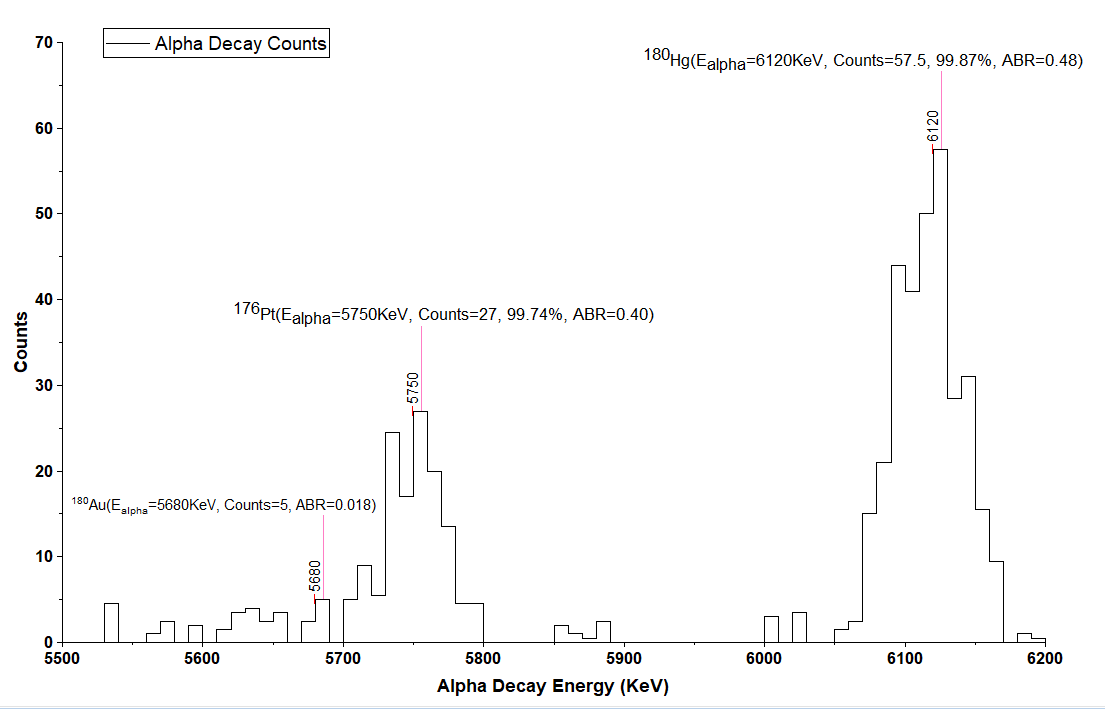
\includegraphics[scale=0.5]{Hg180.png}
%\caption{abcd}
%\label{SignIn Page (i)}
\end{subfigure}
\hfill
\begin{subfigure}
\centering
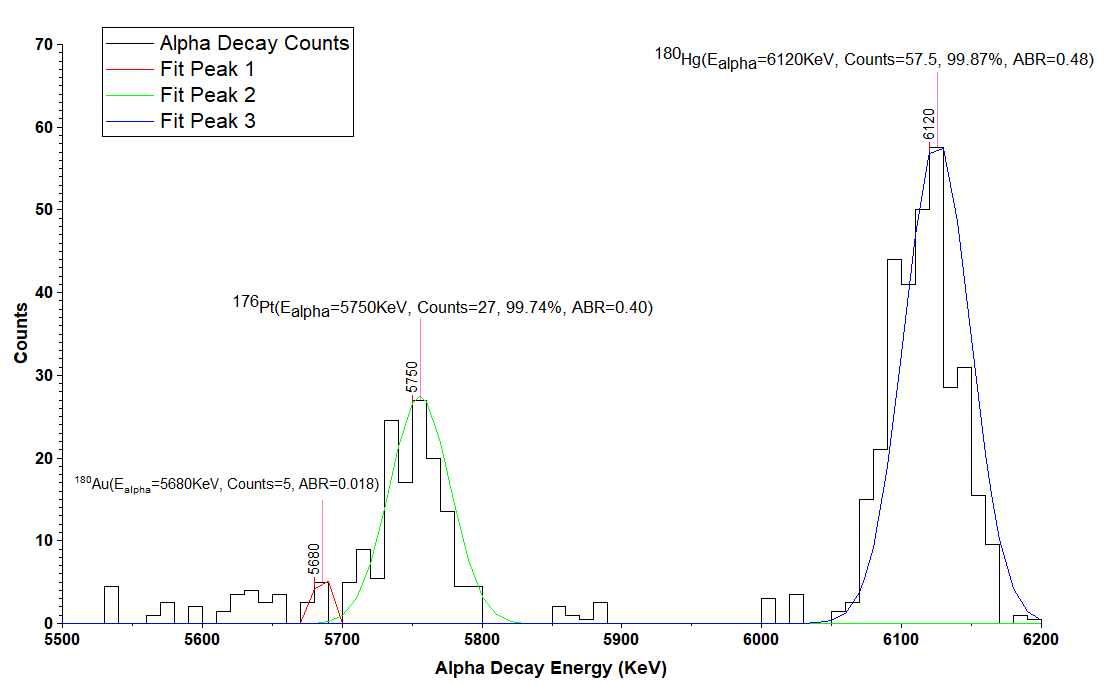
\includegraphics[scale=0.5]{Hg180(Peak Fitting).png}
%\caption{SignIn Page (iii)}
%\label{SignIn Page (iii)}
\end{subfigure}
%\caption{First fig shows the alpha spectrum of $^{180}Hg$ and second fig shows the peak fitting for its prominent peaks.}
\label{First fig shows the alpha spectrum of Hg 180 and second fig shows the peak fitting for its prominent peaks.}
\end{figure}
Here, first fig. shows the alpha spectrum of $^{180}Hg$ while second fig. shows the peak fitting performed for some of its prominent peaks using Gaussian fitting function.
\clearpage

\subsubsection{PRODUCTION OF $^{181}Hg$}
\begin{figure}[h]
\centering
\begin{subfigure}
\centering
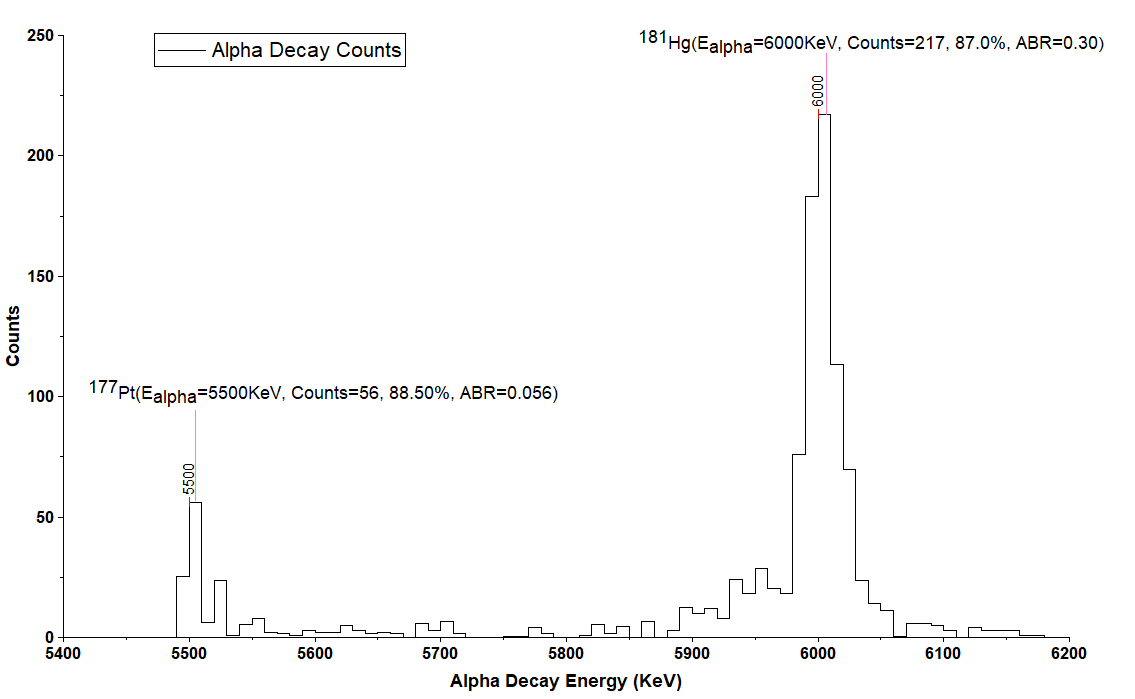
\includegraphics[scale=0.5]{Hg181.png}
%\caption{abcd}
%\label{SignIn Page (i)}
\end{subfigure}
\hfill
\begin{subfigure}
\centering
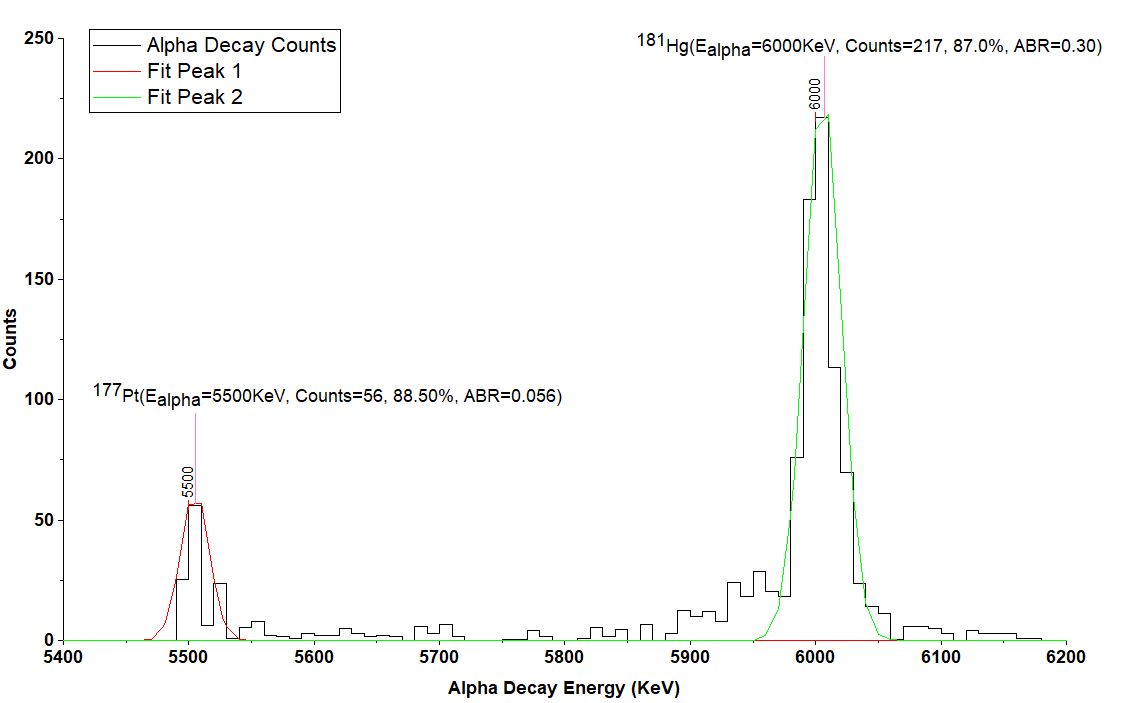
\includegraphics[scale=0.5]{Hg181(Peak Fitting).png}
%\caption{SignIn Page (iii)}
%\label{SignIn Page (iii)}
\end{subfigure}
%\caption{First fig shows the alpha spectrum of $^{180}Hg$ and second fig shows the peak fitting for its prominent peaks.}
\label{First fig shows the alpha spectrum of Hg 181 and second fig shows the peak fitting for its prominent peaks.}
\end{figure}
Here, first fig. shows the alpha spectrum of $^{181}Hg$ while second fig. shows the peak fitting performed for some of its prominent peaks using Gaussian fitting function.
\clearpage

\subsubsection{PRODUCTION OF $^{182}Hg$}
\begin{figure}[h]
\centering
\begin{subfigure}
\centering
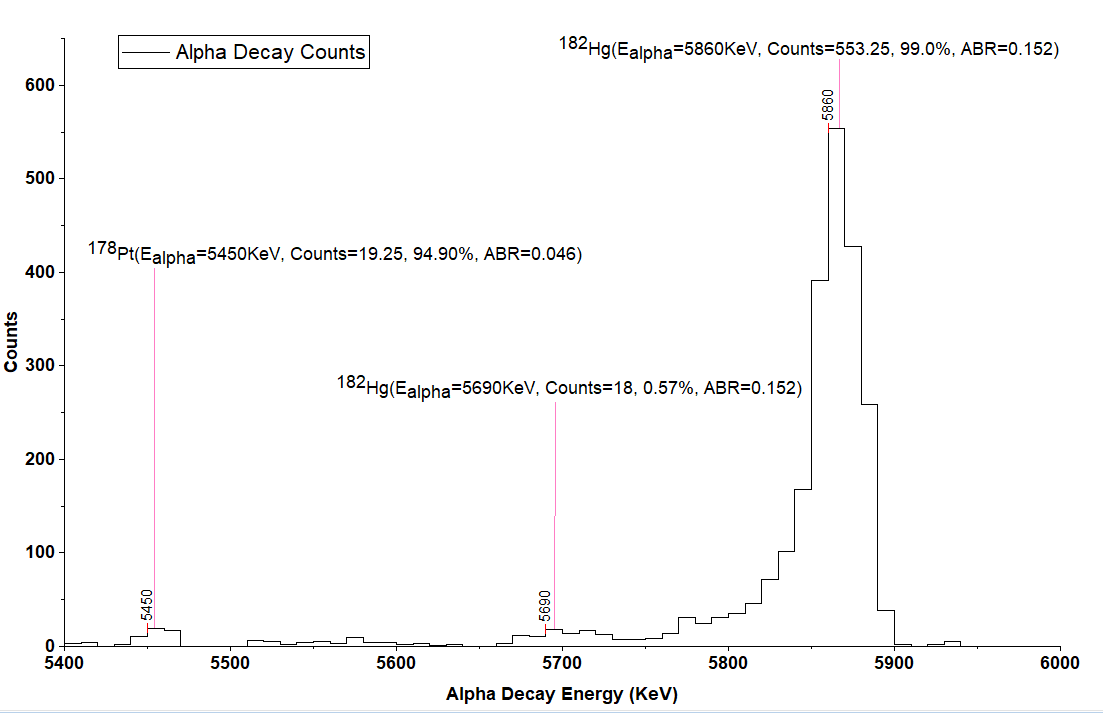
\includegraphics[scale=0.49]{Hg182.png}
%\caption{abcd}
%\label{SignIn Page (i)}
\end{subfigure}
\hfill
\begin{subfigure}
\centering
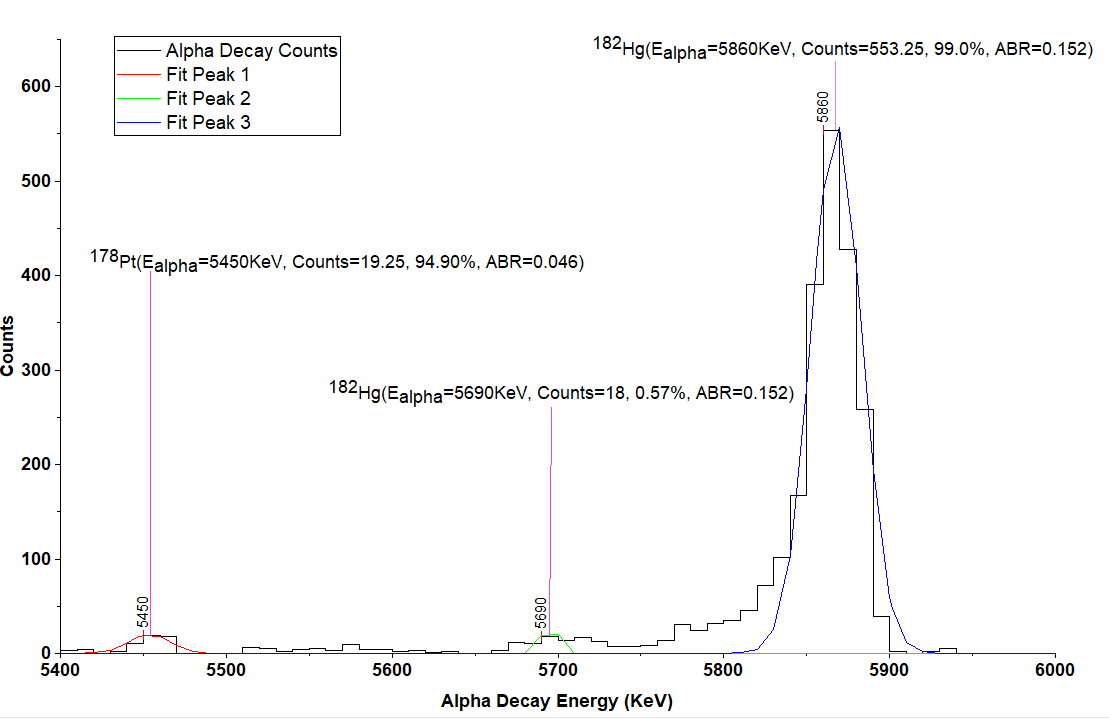
\includegraphics[scale=0.49]{Hg182(Peak Fitting).png}
%\caption{SignIn Page (iii)}
%\label{SignIn Page (iii)}
\end{subfigure}
%\caption{First fig shows the alpha spectrum of $^{180}Hg$ and second fig shows the peak fitting for its prominent peaks.}
\label{First fig shows the alpha spectrum of Hg 182 and second fig shows the peak fitting for its prominent peaks.}
\end{figure}
Here, first fig. shows the alpha spectrum of $^{182}Hg$ while second fig. shows the peak fitting performed for some of its prominent peaks.
\clearpage

\subsubsection{PRODUCTION OF $^{183}Hg$}
\begin{figure}[h]
\centering
\begin{subfigure}
\centering
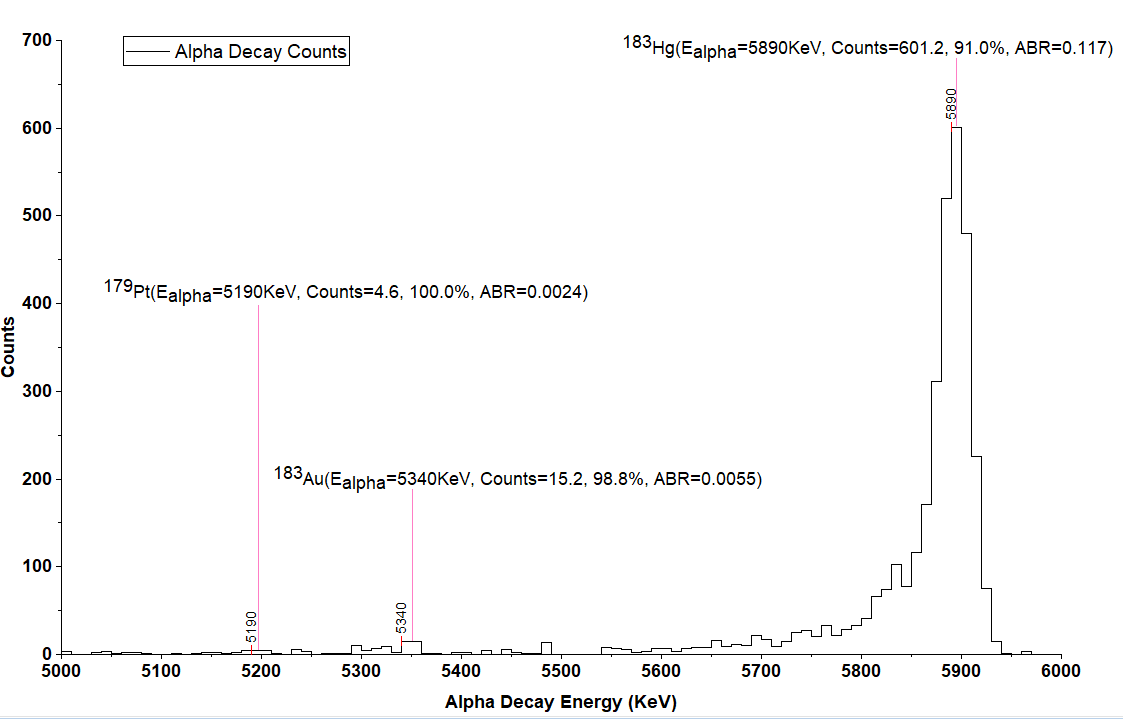
\includegraphics[scale=0.49]{Hg183.png}
%\caption{abcd}
%\label{SignIn Page (i)}
\end{subfigure}
\hfill
\begin{subfigure}
\centering
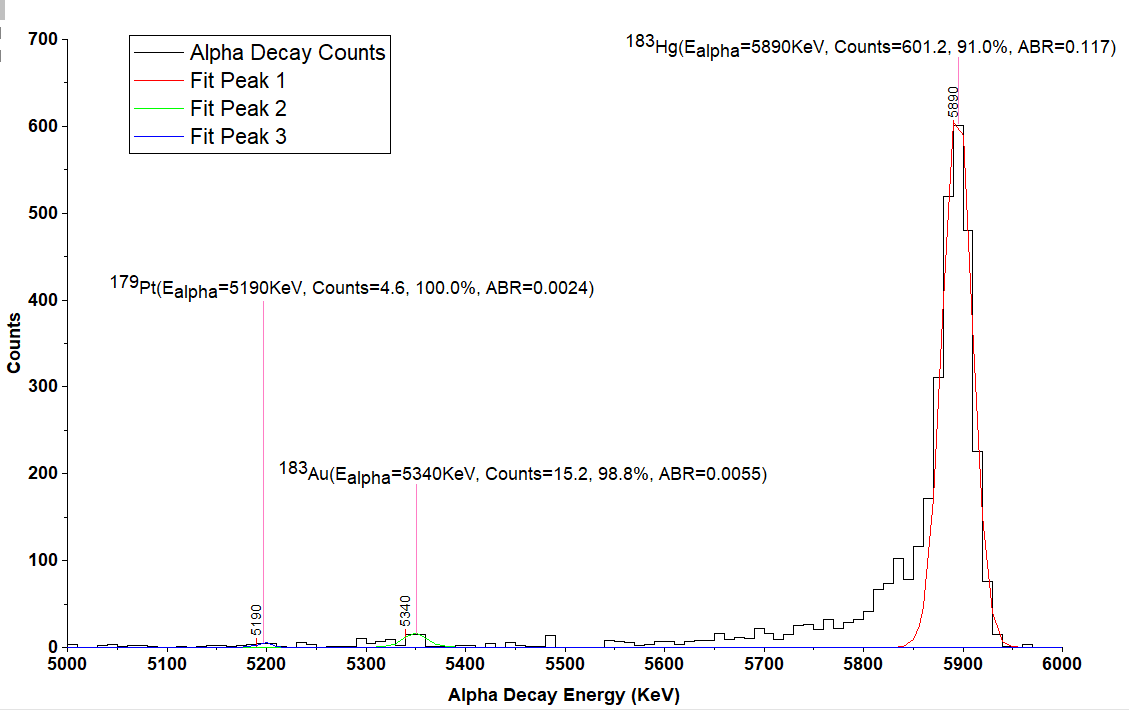
\includegraphics[scale=0.49]{Hg183(Peak Fitting).png}
%\caption{SignIn Page (iii)}
%\label{SignIn Page (iii)}
\end{subfigure}
%\caption{First fig shows the alpha spectrum of $^{180}Hg$ and second fig shows the peak fitting for its prominent peaks.}
\label{First fig shows the alpha spectrum of Hg 183 and second fig shows the peak fitting for its prominent peaks.}
\end{figure}
Here, first fig. shows the alpha spectrum of $^{183}Hg$ while second fig. shows the peak fitting performed for some of its prominent peaks.
\clearpage

\subsubsection{PRODUCTION OF $^{184}Hg$}
\begin{figure}[h]
\centering
\begin{subfigure}
\centering
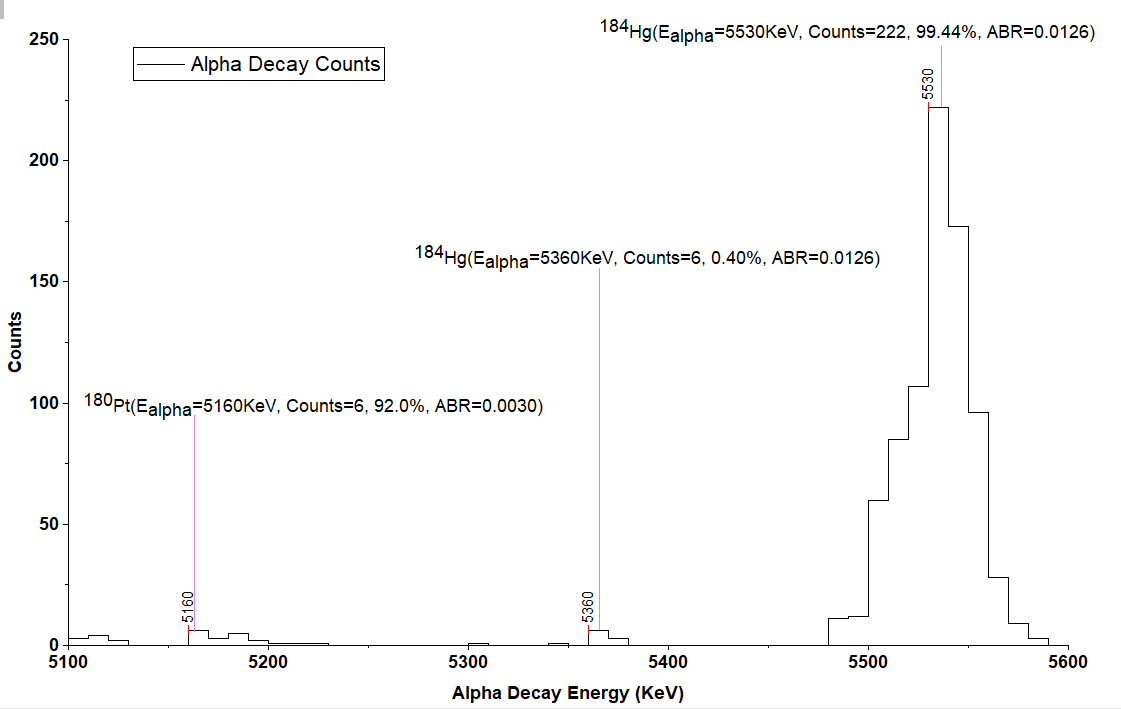
\includegraphics[scale=0.49]{Hg184.png}
%\caption{abcd}
%\label{SignIn Page (i)}
\end{subfigure}
\hfill
\begin{subfigure}
\centering
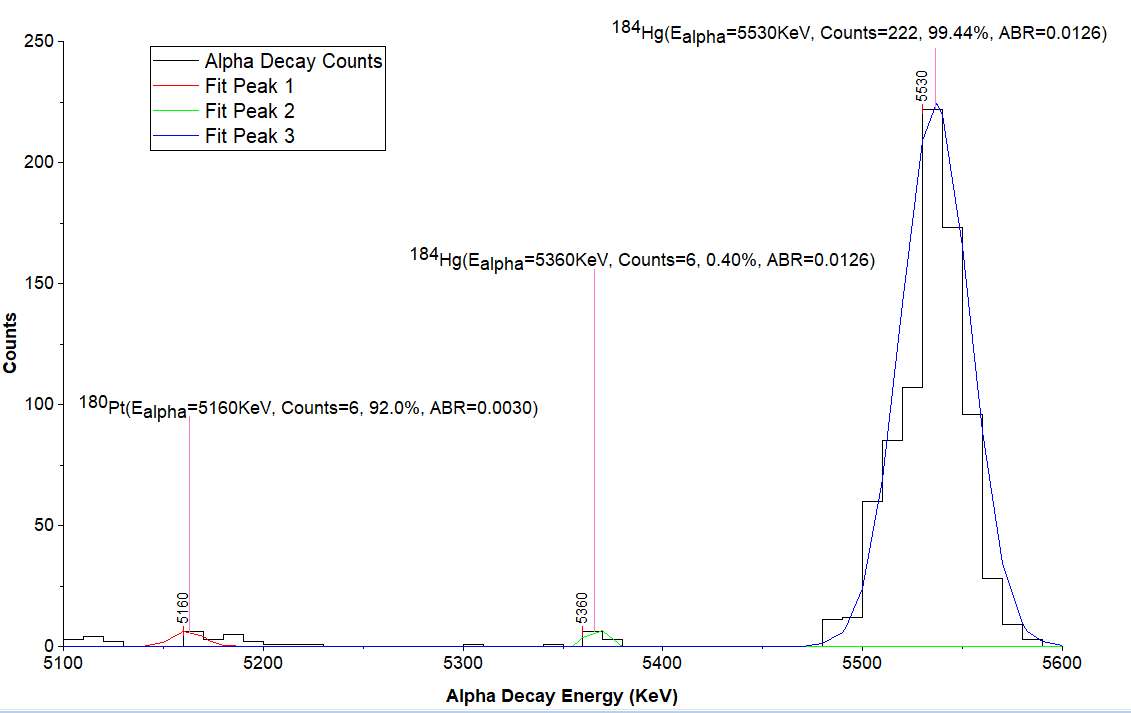
\includegraphics[scale=0.49]{Hg184(Peak Fitting).png}
%\caption{SignIn Page (iii)}
%\label{SignIn Page (iii)}
\end{subfigure}
%\caption{First fig shows the alpha spectrum of $^{180}Hg$ and second fig shows the peak fitting for its prominent peaks.}
\label{First fig shows the alpha spectrum of Hg 184 and second fig shows the peak fitting for its prominent peaks.}
\end{figure}
Here, first fig. shows the alpha spectrum of $^{184}Hg$ while second fig. shows the peak fitting performed for some of its prominent peaks.
\clearpage

\subsubsection{PRODUCTION OF $^{185}Hg$}
\begin{figure}[h]
\centering
\begin{subfigure}
\centering
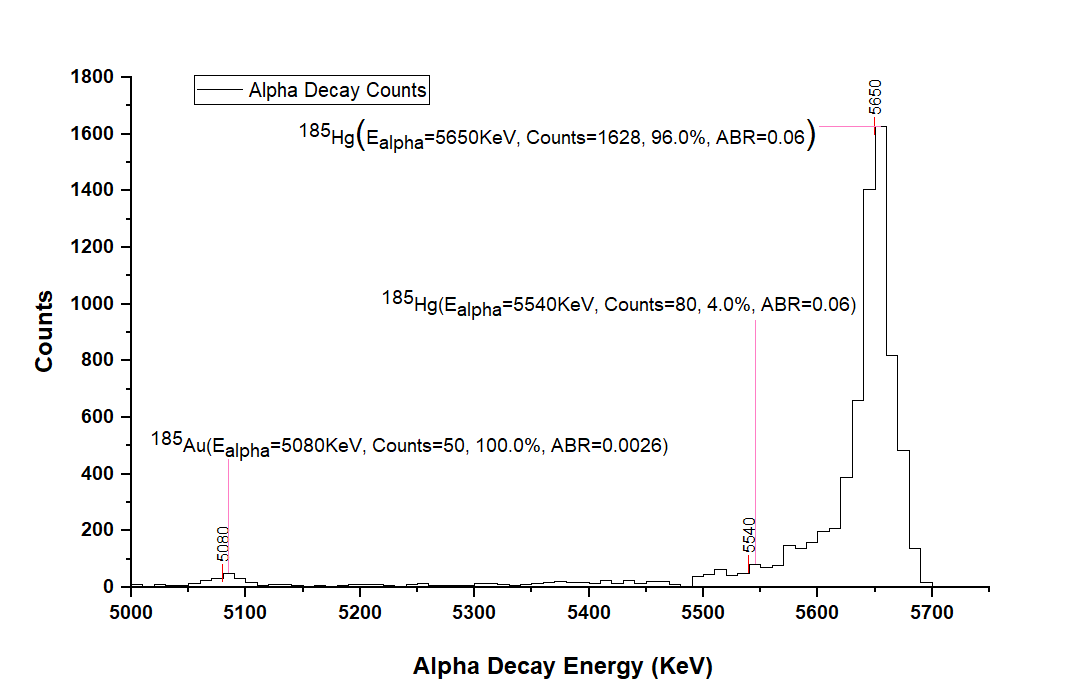
\includegraphics[scale=0.52]{Hg185.png}
%\caption{abcd}
%\label{SignIn Page (i)}
\end{subfigure}
\hfill
\begin{subfigure}
\centering
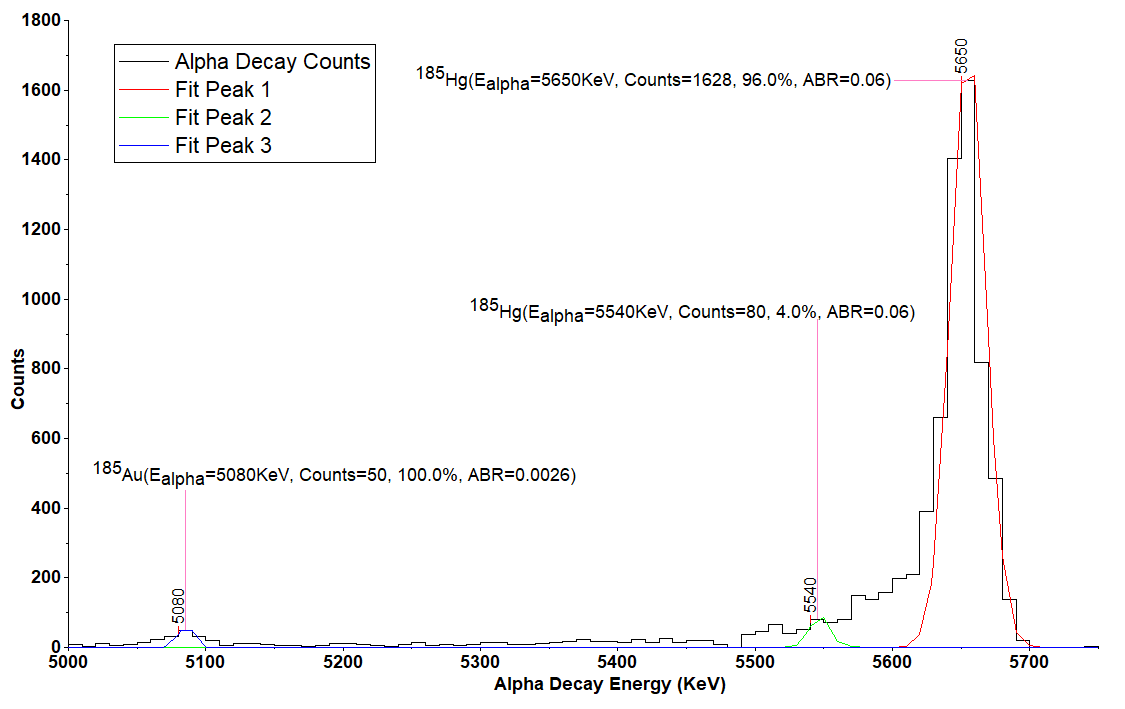
\includegraphics[scale=0.48]{Hg185(Peak Fitting).png}
%\caption{SignIn Page (iii)}
%\label{SignIn Page (iii)}
\end{subfigure}
%\caption{First fig shows the alpha spectrum of $^{180}Hg$ and second fig shows the peak fitting for its prominent peaks.}
\label{First fig shows the alpha spectrum of Hg 185 and second fig shows the peak fitting for its prominent peaks.}
\end{figure}
Here, first fig. shows the alpha spectrum of $^{185}Hg$ while second fig. shows the peak fitting performed for some of its prominent peaks.
\clearpage

\subsubsection{HEATMAP OF Hg ISOTOPES}
\begin{figure}[h]
\centering
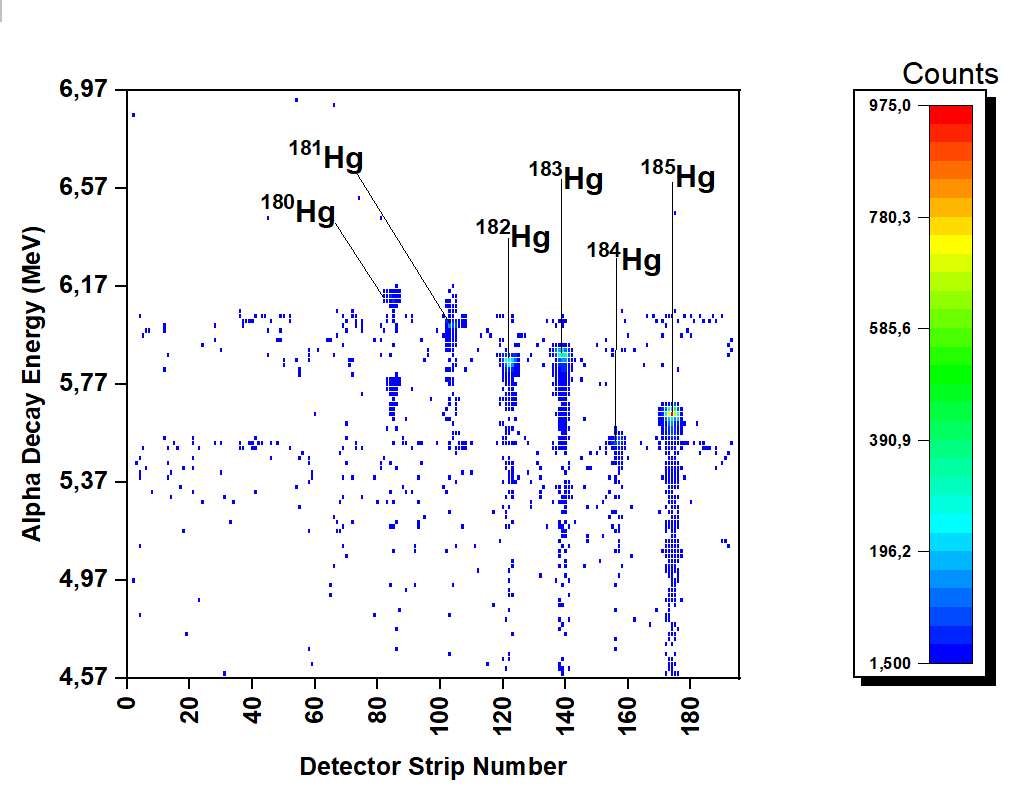
\includegraphics[scale=0.5]{Heatmap_Hg.png}
\caption{\textbf{Heatmap of Hg isotopes.}}
\label{Heatmap of Hg isotopes.}
\end{figure}

\section{SPECTROSCOPIC INVESTIGATION OF\\ RADON ISOTOPES USING FULL-FUSION\\ REACTION $^{166}Er(^{40}Ar,xn)^{206-x}Rn$}
A complete fusion reaction was performed between high energetic projectile particle ($^{40}Ar$) ejected from the window of U-400M cyclotron with an energy \~ 198 MeV and the target material $^{166}Er$ present in the form of rotating disc in the target box of MASHA facility. The products of the nuclear reaction were isotopes of Rn which were detected at focal plane (F2) of the position sensitive Si detector. Further, using the experimental data obtained from the detector and control system of MASHA, their $\alpha$-decay energy spectrum and energy-position graphs were plotted.   
\clearpage

\subsubsection{PRODUCTION OF $^{201}Rn$}
\begin{figure}[h]
\centering
 \begin{subfigure}
\centering
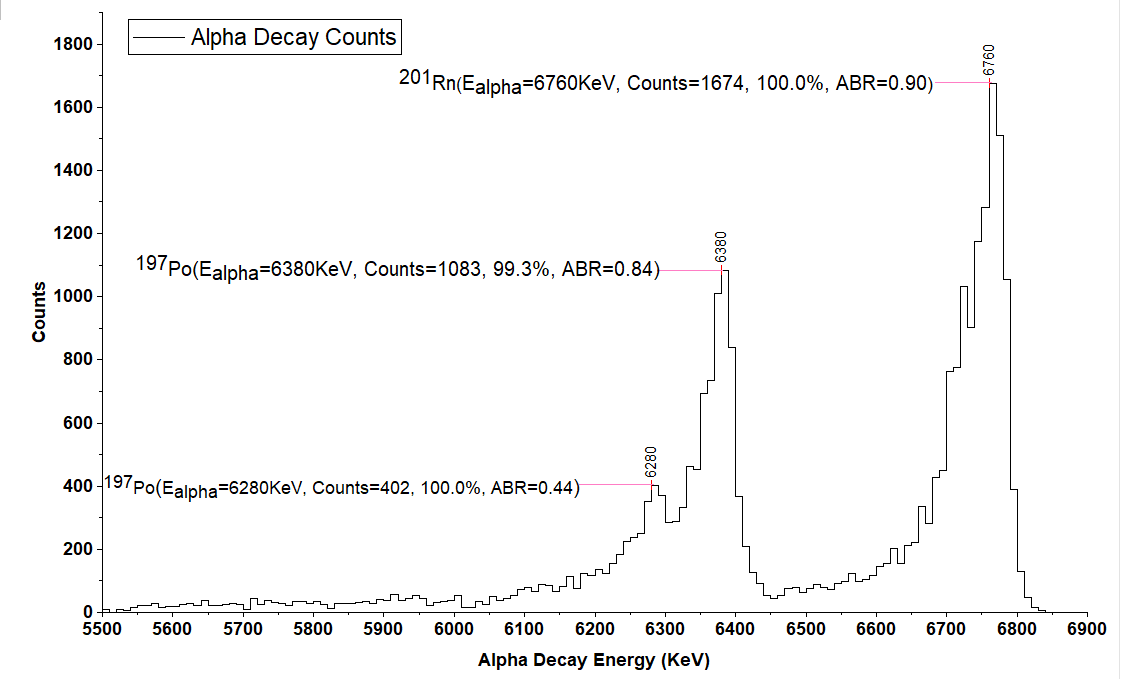
\includegraphics[scale=0.5]{Rn201.png}
%\caption{abcd}
%\label{SignIn Page (i)}
\end{subfigure}
\hfill
\begin{subfigure}
\centering
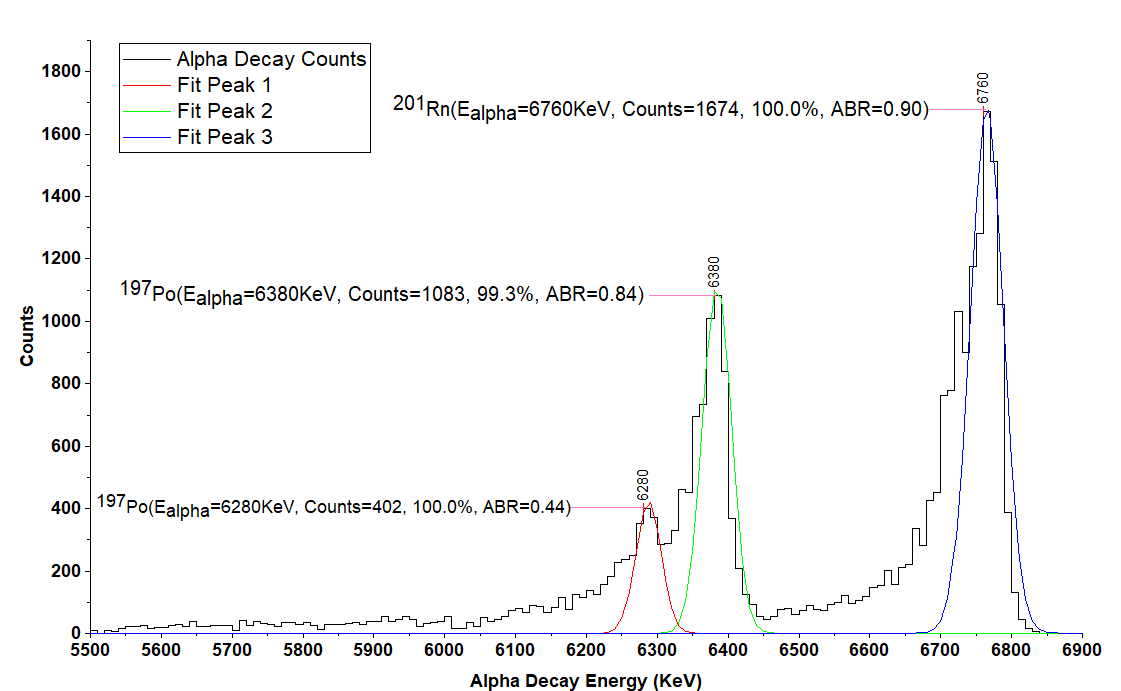
\includegraphics[scale=0.5]{Rn201(Peak Fitting).png}
%\caption{SignIn Page (iii)}
%\label{SignIn Page (iii)}
\end{subfigure}
%\caption{First fig shows the alpha spectrum of $^{180}Hg$ and second fig shows the peak fitting for its prominent peaks.}
\label{First fig shows the alpha spectrum of Rn 201 and second fig shows the peak fitting for its prominent peaks.}
\end{figure}
Here, first fig. shows the alpha spectrum of $^{201}Rn$ while second fig. shows the peak fitting performed for some of its prominent peaks using Gaussian fitting function.
\clearpage

\subsubsection{PRODUCTION OF $^{202}Rn$}
\begin{figure}[h]
\centering
 \begin{subfigure}
\centering
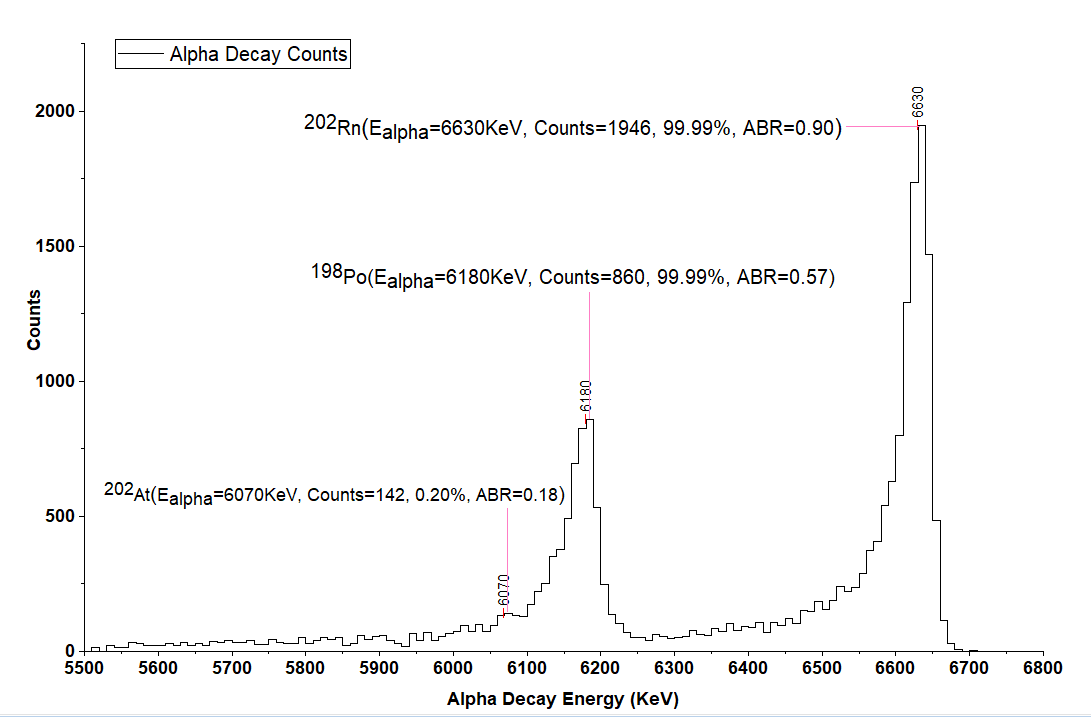
\includegraphics[scale=0.49]{Rn202.png}
%\caption{abcd}
%\label{SignIn Page (i)}
\end{subfigure}
\hfill
\begin{subfigure}
\centering
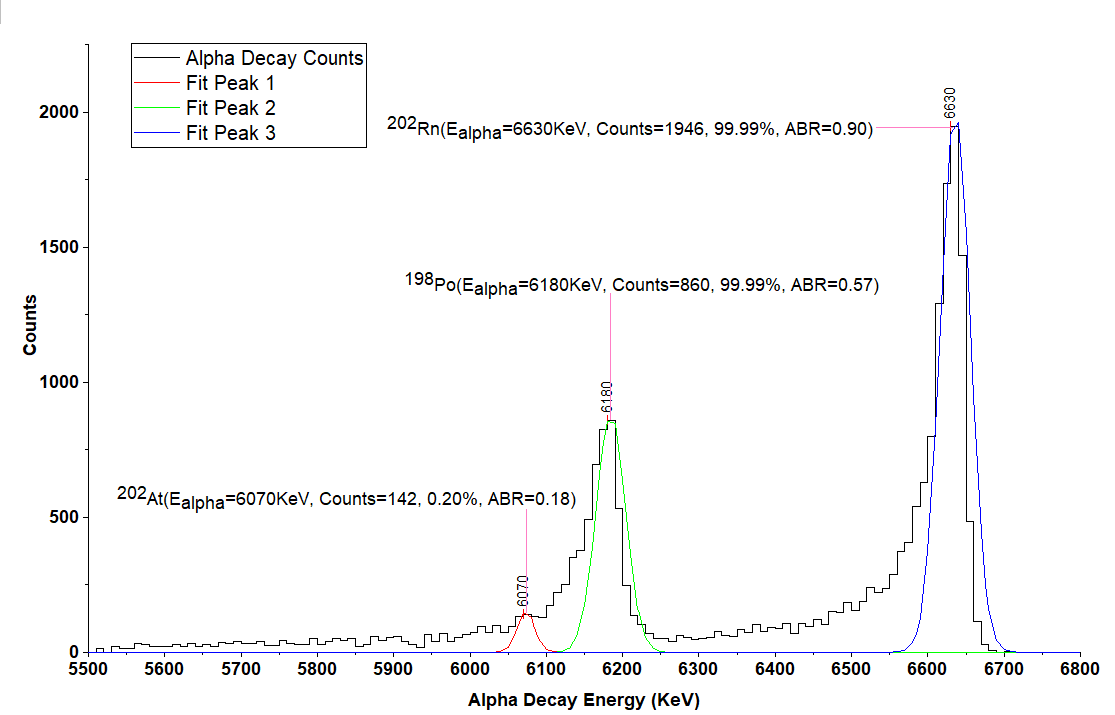
\includegraphics[scale=0.49]{Rn202(Peak Fitting).png}
%\caption{SignIn Page (iii)}
%\label{SignIn Page (iii)}
\end{subfigure}
%\caption{First fig shows the alpha spectrum of $^{180}Hg$ and second fig shows the peak fitting for its prominent peaks.}
\label{First fig shows the alpha spectrum of Rn 202 and second fig shows the peak fitting for its prominent peaks.}
\end{figure}
Here, first fig. shows the alpha spectrum of $^{202}Rn$ while second fig. shows the peak fitting performed for some of its prominent peaks.
\clearpage

\subsubsection{PRODUCTION OF $^{203}Rn$}
\begin{figure}[h]
\centering
 \begin{subfigure}
\centering
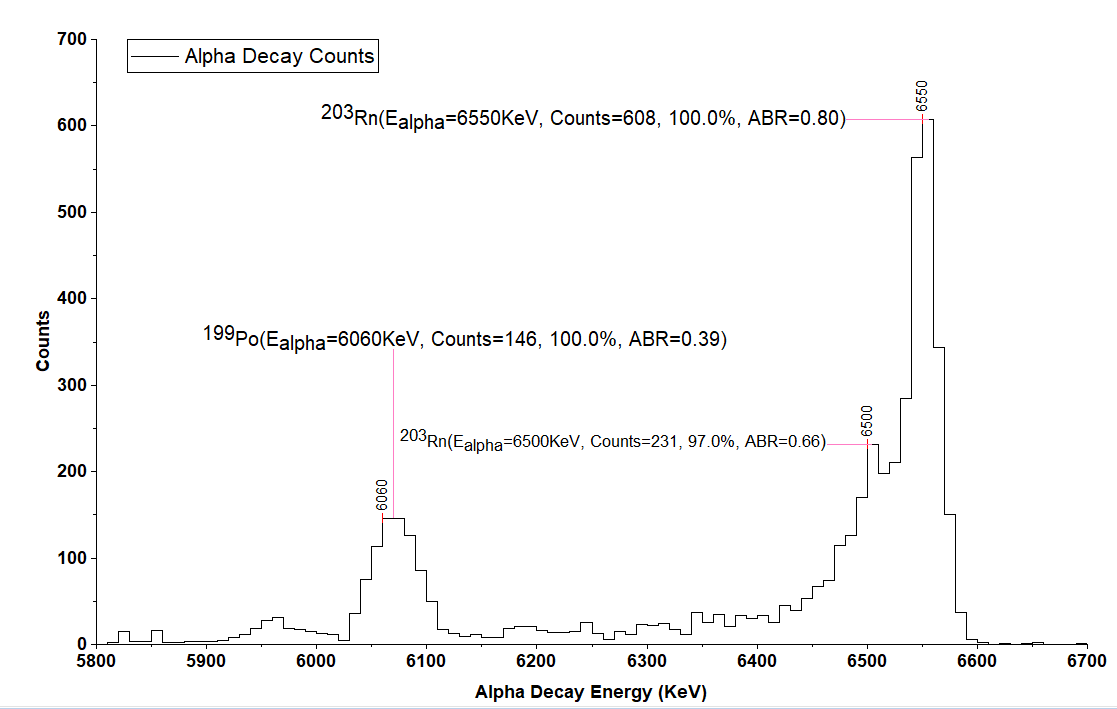
\includegraphics[scale=0.49]{Rn203.png}
%\caption{abcd}
%\label{SignIn Page (i)}
\end{subfigure}
\hfill
\begin{subfigure}
\centering
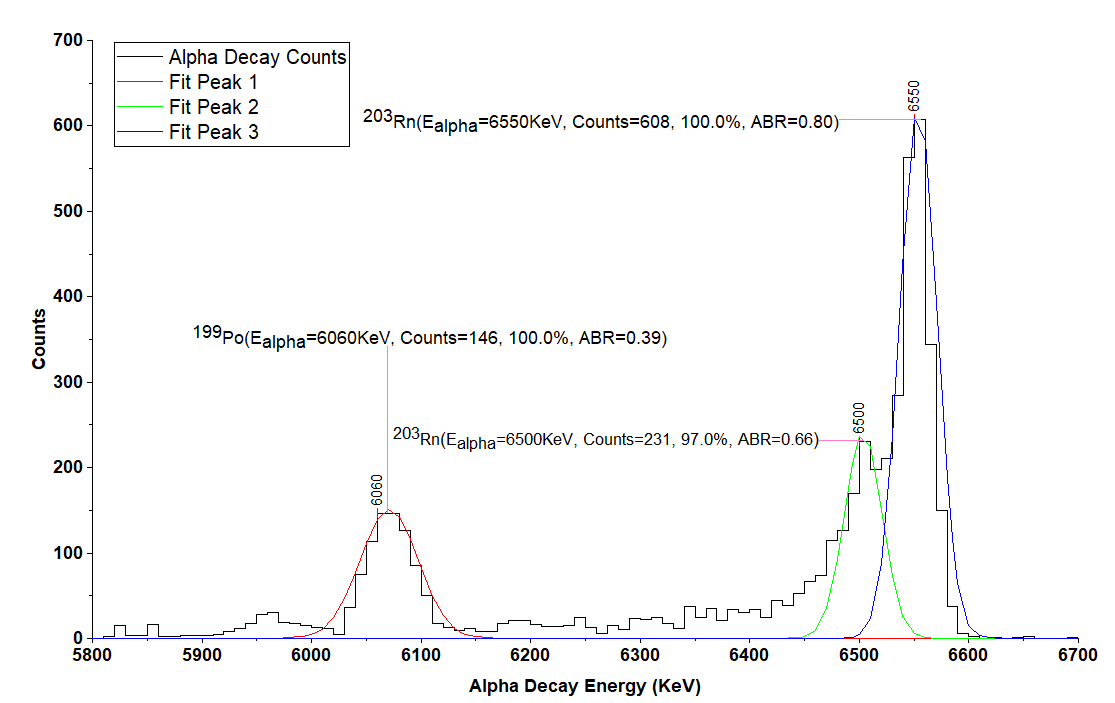
\includegraphics[scale=0.49]{Rn203(Peak Fitting).png}
%\caption{SignIn Page (iii)}
%\label{SignIn Page (iii)}
\end{subfigure}
%\caption{First fig shows the alpha spectrum of $^{180}Hg$ and second fig shows the peak fitting for its prominent peaks.}
\label{First fig shows the alpha spectrum of Rn 203 and second fig shows the peak fitting for its prominent peaks.}
\end{figure}
Here, first fig. shows the alpha spectrum of $^{203}Rn$ while second fig. shows the peak fitting performed for some of its prominent peaks.
\clearpage

\subsubsection{PRODUCTION OF $^{204}Rn$}
\begin{figure}[h]
\centering
 \begin{subfigure}
\centering
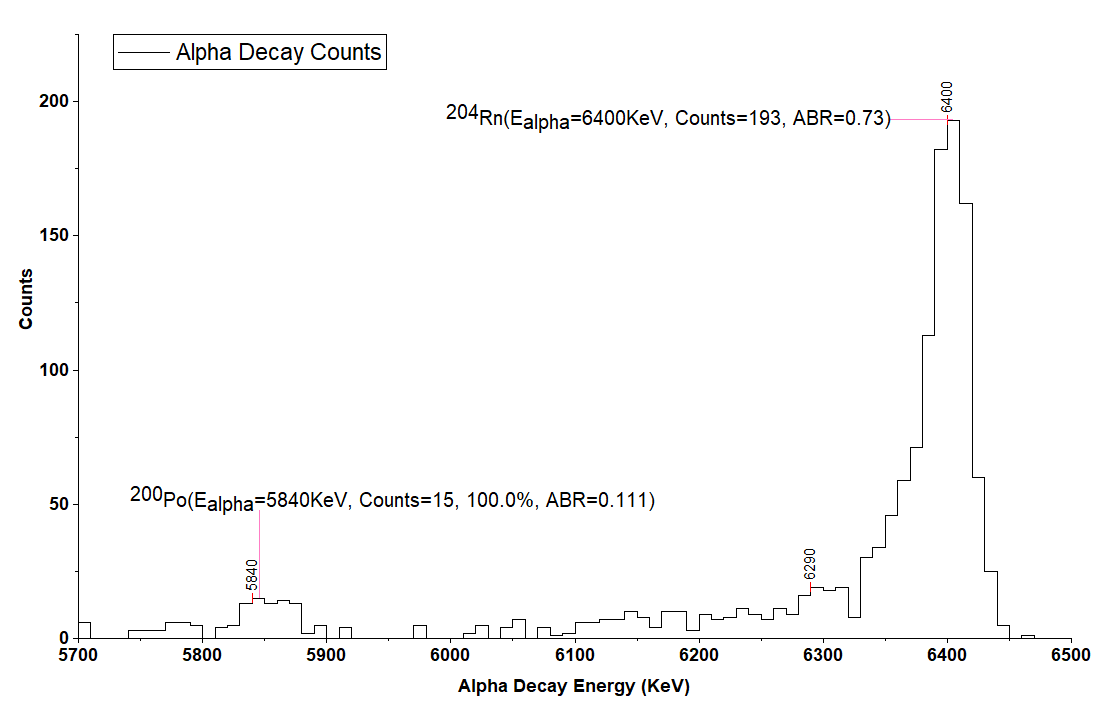
\includegraphics[scale=0.5]{Rn204.png}
%\caption{abcd}
%\label{SignIn Page (i)}
\end{subfigure}
\hfill
\begin{subfigure}
\centering
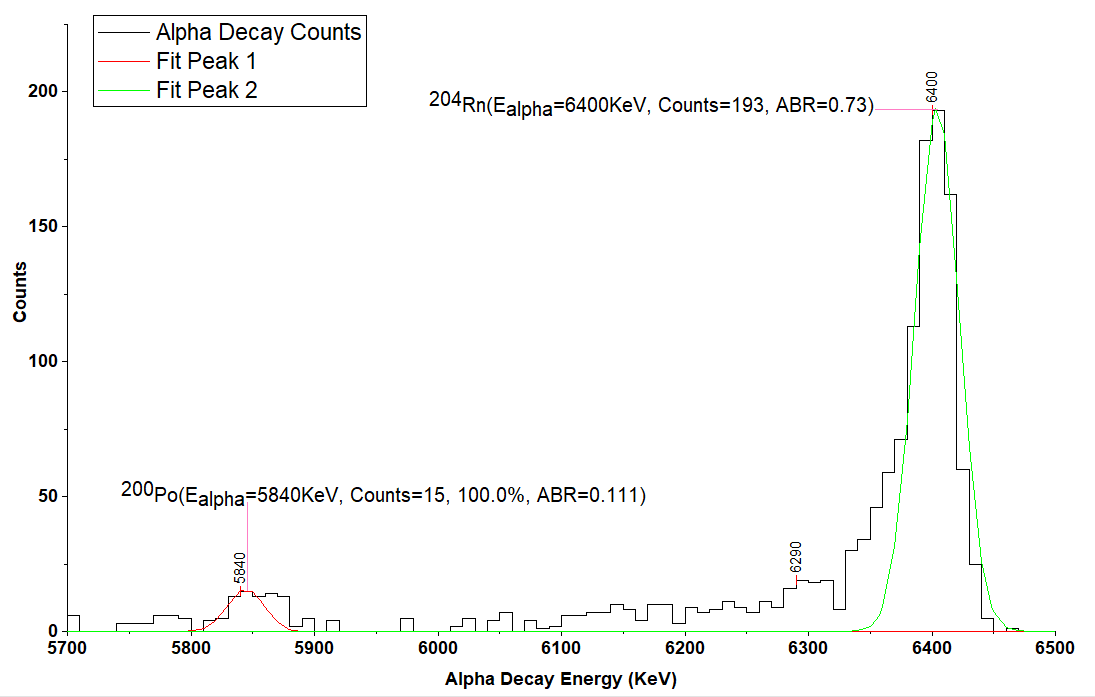
\includegraphics[scale=0.5]{Rn204(Peak Fitting).png}
%\caption{SignIn Page (iii)}
%\label{SignIn Page (iii)}
\end{subfigure}
%\caption{First fig shows the alpha spectrum of $^{180}Hg$ and second fig shows the peak fitting for its prominent peaks.}
\label{First fig shows the alpha spectrum of Rn 204 and second fig shows the peak fitting for its prominent peaks.}
\end{figure}
Here, first fig. shows the alpha spectrum of $^{204}Rn$ while second fig. shows the peak fitting performed for some of its prominent peaks using Gaussian fitting function.
\clearpage

\subsubsection{PRODUCTION OF $^{205}Rn$}
\begin{figure}[h]
\centering
 \begin{subfigure}
\centering
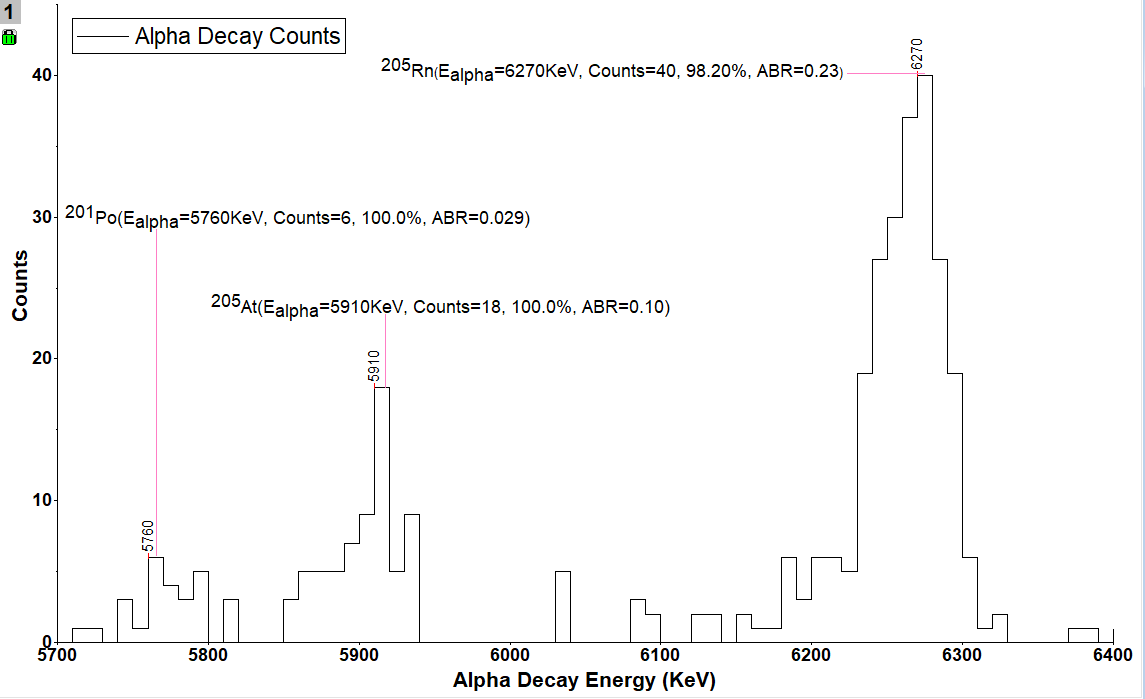
\includegraphics[scale=0.5]{Rn205.png}
%\caption{abcd}
%\label{SignIn Page (i)}
\end{subfigure}
\hfill
\begin{subfigure}
\centering
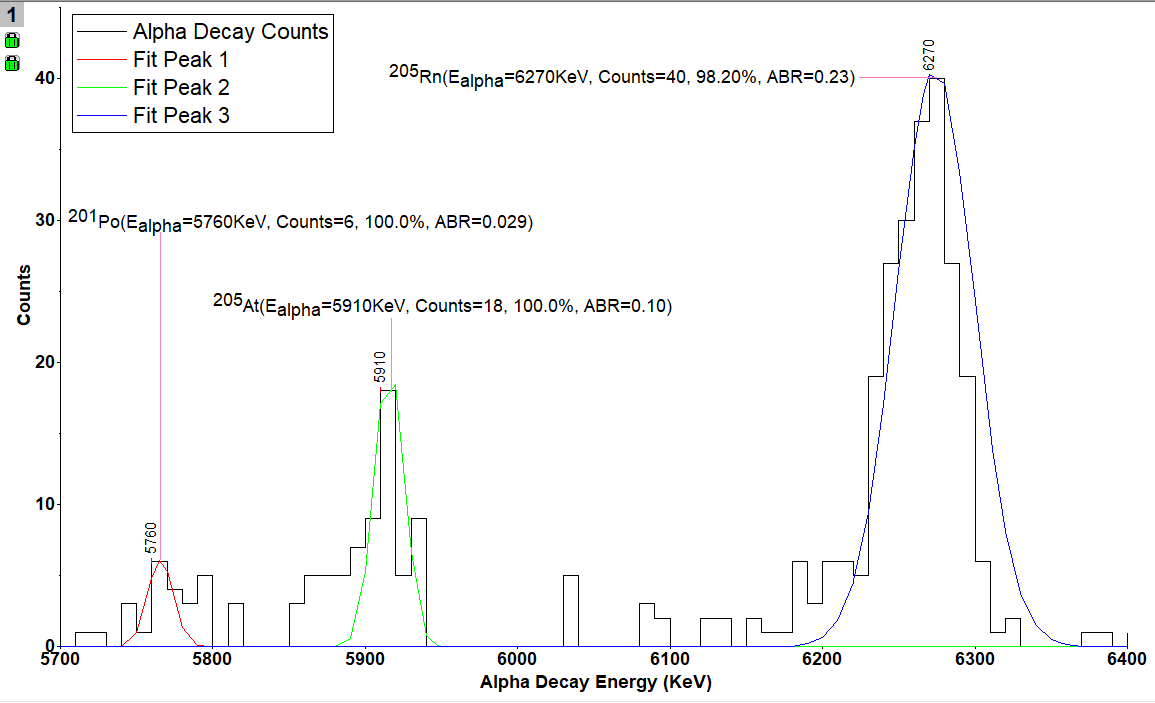
\includegraphics[scale=0.5]{Rn205(Peak Fitting).png}
%\caption{SignIn Page (iii)}
%\label{SignIn Page (iii)}
\end{subfigure}
%\caption{First fig shows the alpha spectrum of $^{180}Hg$ and second fig shows the peak fitting for its prominent peaks.}
\label{First fig shows the alpha spectrum of Rn 205 and second fig shows the peak fitting for its prominent peaks.}
\end{figure}
Here, first fig. shows the alpha spectrum of $^{205}Rn$ while second fig. shows the peak fitting performed for some of its prominent peaks using Gaussian fitting function.
\clearpage

\subsubsection{HEATMAP OF Rn ISOTOPES ($^{166}Er(^{40}Ar,xn)^{206-x}Rn$)}
\begin{figure}[h]
\centering
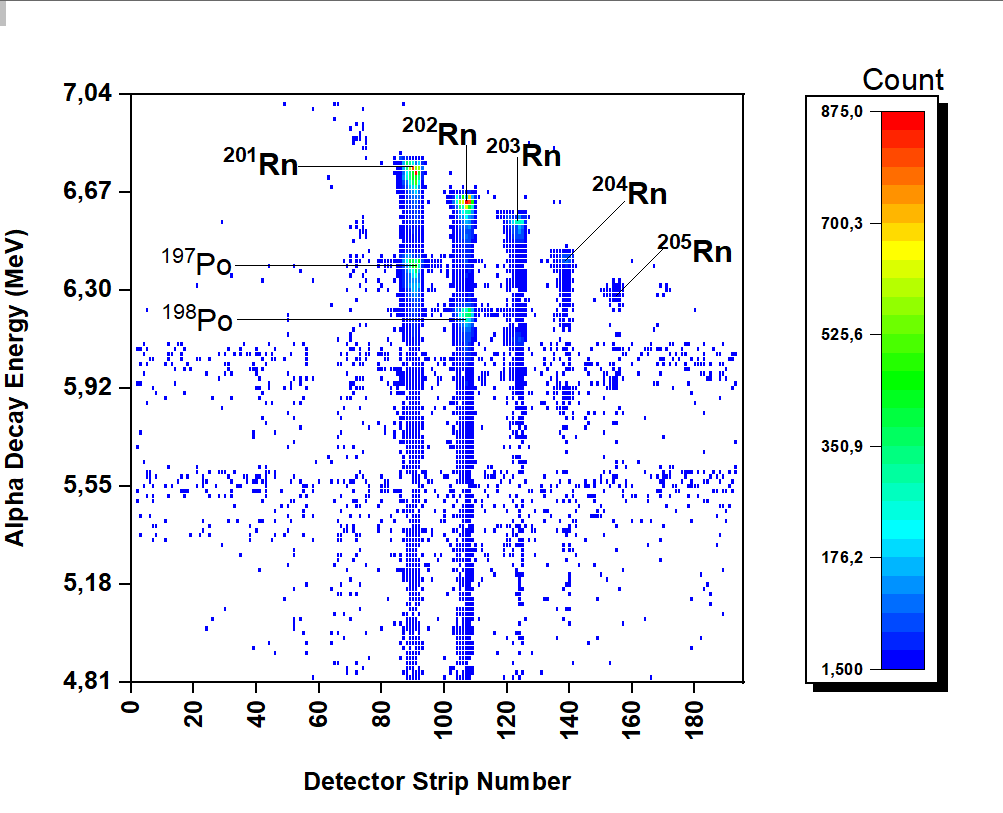
\includegraphics[scale=0.5]{Heatmap_Rn(201-205).png}
\caption{\textbf{Heatmap of Rn isotopes using complete-fusion reaction $^{166}Er(^{40}Ar,xn)^{206-x}Rn$.}}
\label{Heatmap of Rn(201-205) isotopes.}
\end{figure}

\section{SPECTROSCOPIC INVESTIGATION OF RADON ISOTOPES USING MNTR\\ $^{48}Ca$ + $^{242}Pu$}
Unlike complete fusion reactions discussed above, a MNTR can have any possible product nucleus. However, in the reaction of ${48}Ca$ + $^{242}Pu$ under some fixed conditions, new neutron-rich Rn isotopes were produced near the neutron N=126 shell closure configuration, using MNTR. The isotopes produced were identified first, later their spectroscopic investigations were carried out. However, it was observed that only those Rn isotopes reached the detector and were identified which lived at least 35 ms while others decayed in their path. 

\clearpage

\subsubsection{PRODUCTION OF $^{212}Rn$}
\begin{figure}[h]
\centering
 \begin{subfigure}
\centering
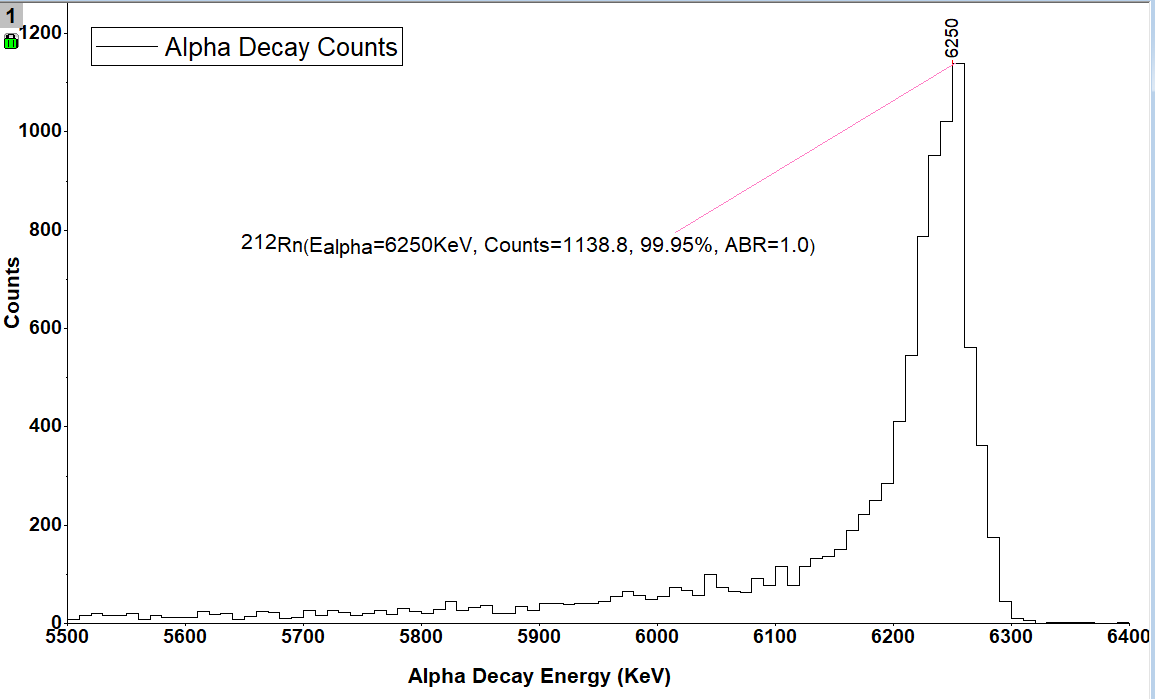
\includegraphics[scale=0.5]{Rn212.png}
%\caption{abcd}
%\label{SignIn Page (i)}
\end{subfigure}
\hfill
\begin{subfigure}
\centering
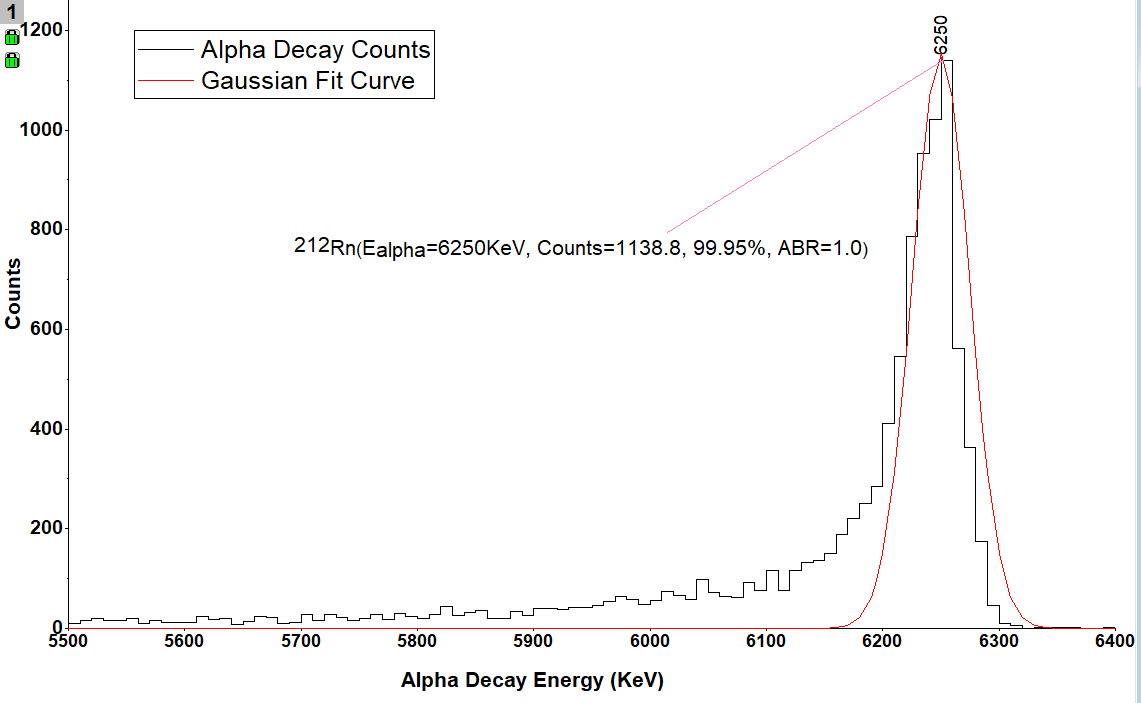
\includegraphics[scale=0.5]{Rn212(Peak Fitting).png}
%\caption{SignIn Page (iii)}
%\label{SignIn Page (iii)}
\end{subfigure}
%\caption{First fig shows the alpha spectrum of $^{180}Hg$ and second fig shows the peak fitting for its prominent peaks.}
\label{First fig shows the alpha spectrum of Rn 212 and second fig shows the peak fitting for its prominent peaks.}
\end{figure}
Here, first fig. shows the alpha spectrum of $^{212}Rn$ while second fig. shows the peak fitting performed for some of its prominent peaks using Gaussian fitting function.
\clearpage

\subsubsection{PRODUCTION OF $^{218}Rn$}
\begin{figure}[h]
\centering
 \begin{subfigure}
\centering
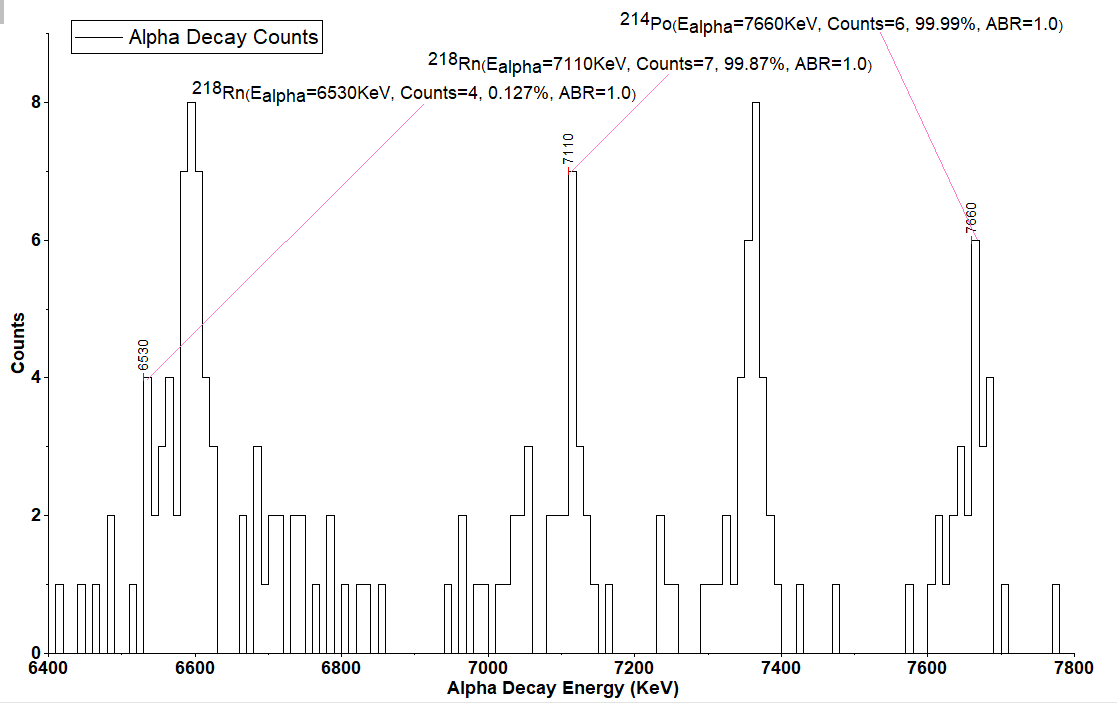
\includegraphics[scale=0.5]{Rn218.png}
%\caption{abcd}
%\label{SignIn Page (i)}
\end{subfigure}
\hfill
\begin{subfigure}
\centering
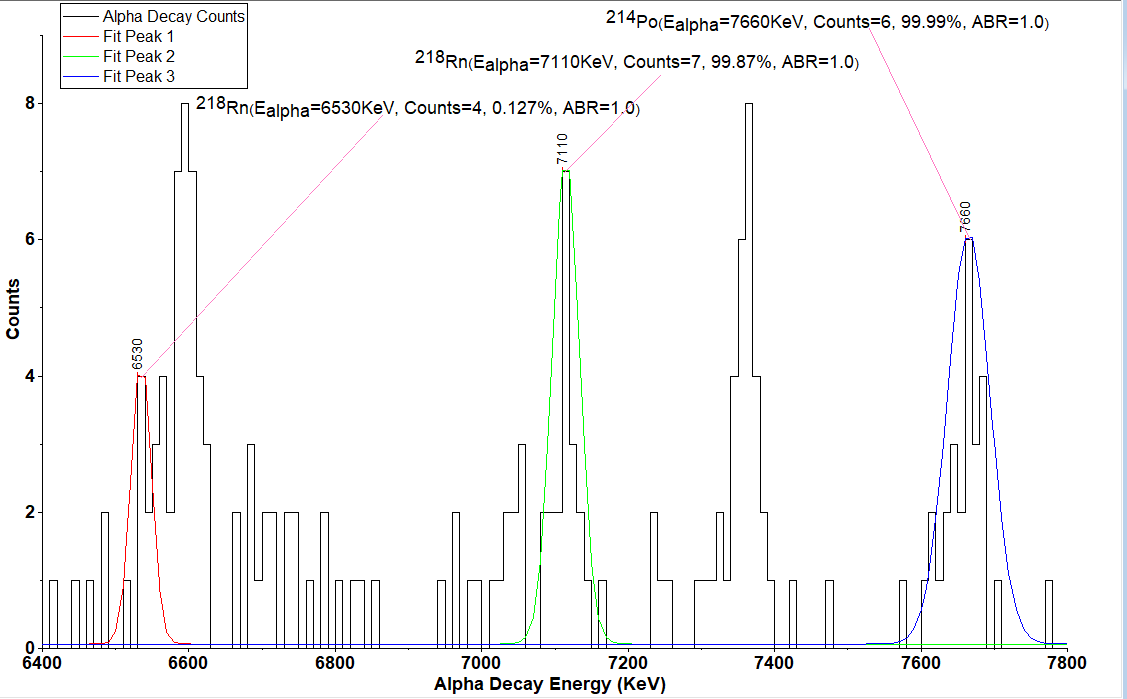
\includegraphics[scale=0.5]{Rn218(Peak Fitting).png}
%\caption{SignIn Page (iii)}
%\label{SignIn Page (iii)}
\end{subfigure}
%\caption{First fig shows the alpha spectrum of $^{180}Hg$ and second fig shows the peak fitting for its prominent peaks.}
\label{First fig shows the alpha spectrum of Rn 218 and second fig shows the peak fitting for its prominent peaks.}
\end{figure}
Here, first fig. shows the alpha spectrum of $^{218}Rn$ while second fig. shows the peak fitting performed for some of its prominent peaks using Gaussian fitting function.
\clearpage

\subsubsection{PRODUCTION OF $^{219}Rn$}
\begin{figure}[h]
\centering
 \begin{subfigure}
\centering
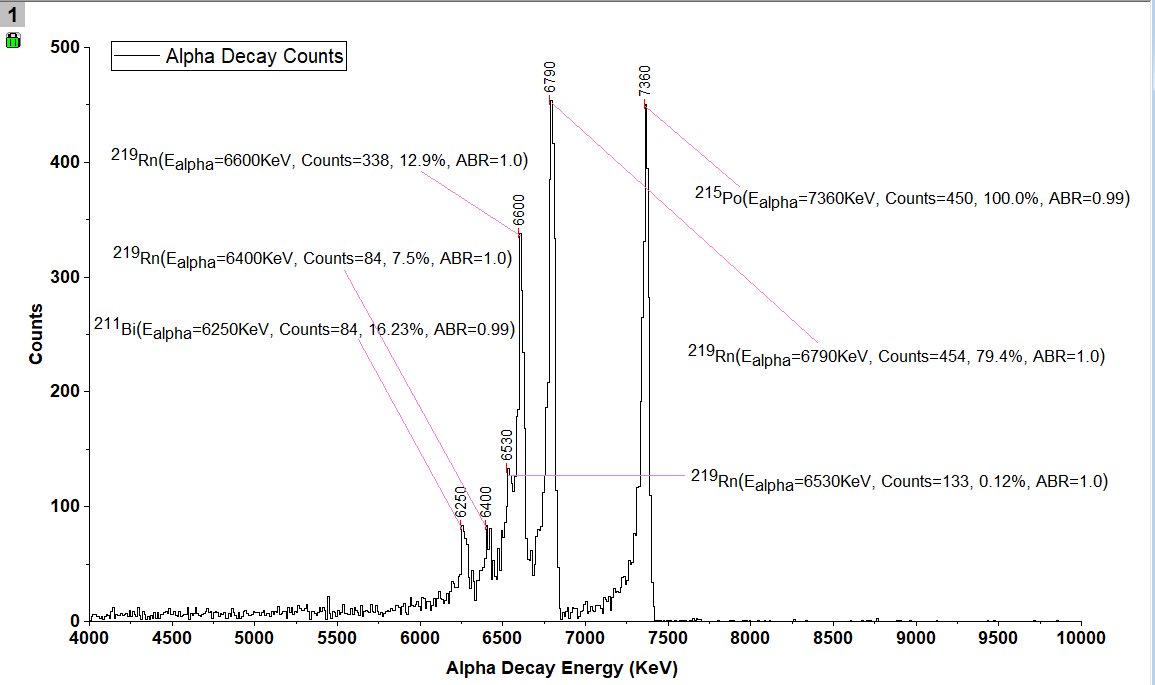
\includegraphics[scale=0.5]{Rn219.png}
%\caption{abcd}
%\label{SignIn Page (i)}
\end{subfigure}
\hfill
\begin{subfigure}
\centering
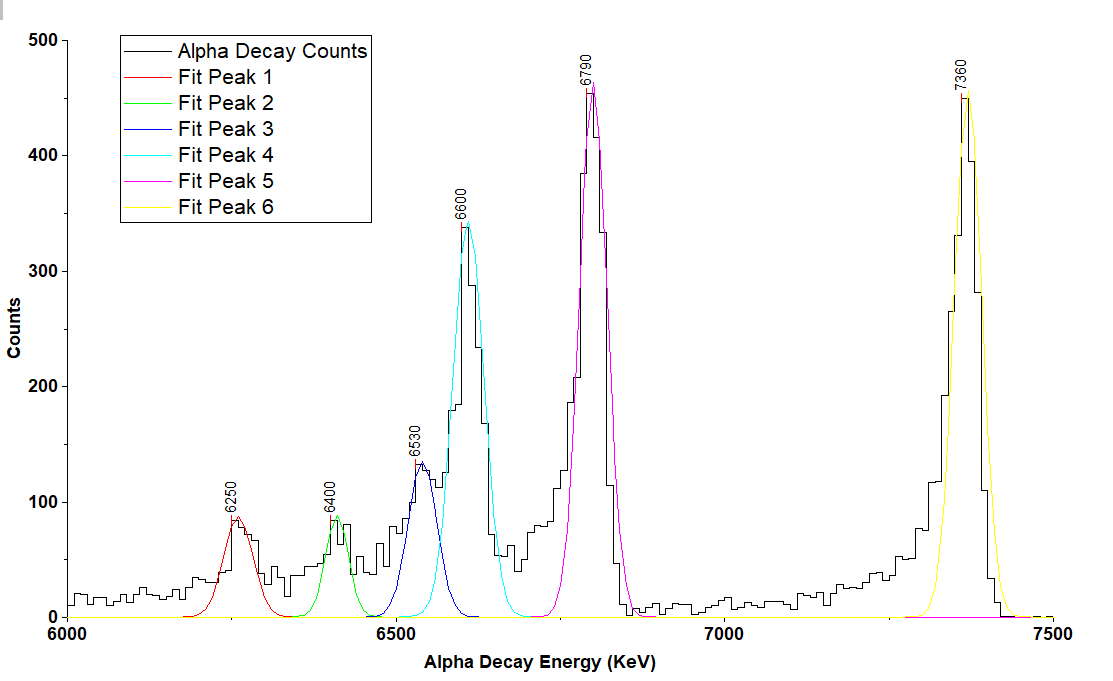
\includegraphics[scale=0.5]{Rn219(Peak Fitting).png}
%\caption{SignIn Page (iii)}
%\label{SignIn Page (iii)}
\end{subfigure}
%\caption{First fig shows the alpha spectrum of $^{180}Hg$ and second fig shows the peak fitting for its prominent peaks.}
\label{First fig shows the alpha spectrum of Rn 219 and second fig shows the peak fitting for its prominent peaks.}
\end{figure}
Here, first fig. shows the alpha spectrum of $^{219}Rn$ while second fig. shows the peak fitting performed for some of its prominent peaks using Gaussian fitting function.
\clearpage

\subsubsection{HEATMAP OF Rn ISOTOPES ($^{48}Ca$ + $^{242}Pu$)}
\begin{figure}[h]
\centering
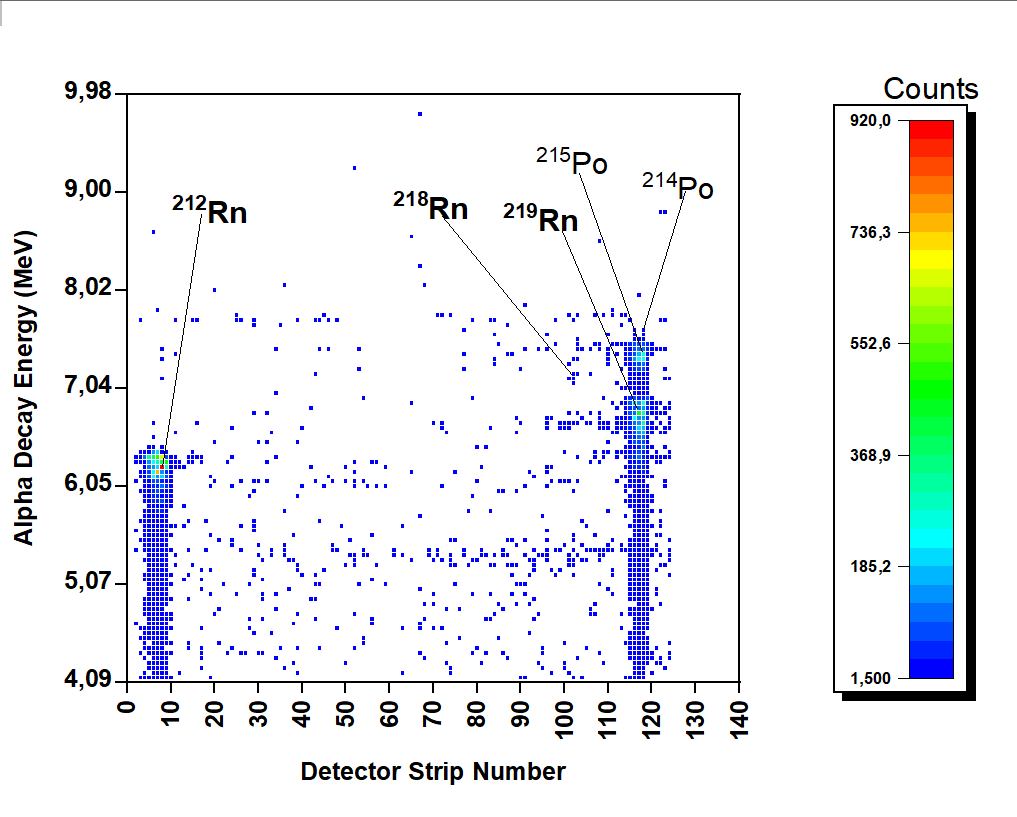
\includegraphics[scale=0.5]{Heatmap_Rn(212,218,219).png}
\caption{\textbf{Heatmap of Rn isotopes using MNTR $^{48}Ca$ + $^{242}Pu$.}}
\label{Heatmap of Rn(212, 218, 219) isotopes.}
\end{figure}

\section{RESULTS AND CONCLUSIONS}
In this work we have studied about the production and spectroscopic investigation of Hg and Rn isotopes using full fusion reactions $^{40}Ar$ + $^{148}Sm$ $\rightarrow$ $^{188-x}Hg$ + $xn$, $^{40}Ar$ + $^{166}Er$ $\rightarrow$ $^{206-x}Rn$ + $xn$  and MNTR $^{48}Ca$ + $^{242}Pu$. The final product in all these reactions were isotopes of Hg and Rn. The experimental data obtained from the MASHA were analyzed and 1D $\alpha$-decay energy spectrum graph was plotted for those strips of detector which had detected any isotopic product of nuclear reaction. Further, we used this 1D histograms to plot a 2D energy-position graph, separately for Hg and Rn isotopes. We have identified the masses of super-heavy nuclei which were detected at different strips of Si based Position Sensitive Detector (PSD). Using 1D histograms and nuclide chart, we have also calculated their $E_a$, ABR, Counts, and their probability to decay with a specific amount of energy.

\section{ACKNOWLEDGEMENT}
Firstly, I would thank my scientific supervisor Mr. Viacheslav Vedeneev for giving me this wonderful opportunity to work on a research project under his guidance. He guided me throughout the duration of this project and even helped me to excel in Origin. I would also like to thank the whole INTEREST team for their constant support and making the application process smooth. I would even thank my parents and my elder brother for continuously motivating me to complete this project successfully. 

\bibliographystyle{apacite}
\bibliography{Ref}
\end{document}
